\documentclass[twoside,AutoFakeBold=true]{ZJUthesisv2}
% 该文档中首字符为“%”的均为注释行,不会在论文中出现
% 论文默认为双面模式,需单面模式请将第一行换为如下所示:
% \documentclass[oneside]{ZJUthesis}
% \documentclass[twoside]{ZJUthesis}

% 取消目录中链接的颜色,方便打印
% 如需颜色,请将“false”改为“true”
%\usepackage{hyperref}
\hypersetup{colorlinks=false}

% 这里几行代码使得目录中的“第几章” 和后面的章节名称不致发生重叠
\makeatletter
\renewcommand{\numberline}[1]{%
\settowidth\@tempdimb{#1\hspace{0.5em}}%
\ifdim\@tempdima<\@tempdimb%
  \@tempdima=\@tempdimb%
\fi%
\hb@xt@\@tempdima{\@cftbsnum #1\@cftasnum\hfil}\@cftasnumb}
\makeatother

%\usepackage[sectionbib]{chapterbib}

% \makeatletter
% \def\@chapter[#1]#2{\ifnum \c@secnumdepth >\m@ne
%   \if@mainmatter
%     \refstepcounter{chapter}%
%     \typeout{\@chapapp\space\thechapter.}%
%     \addcontentsline{toc}{chapter}%
%     {\protect\numberline{第 \chaptername 章}\hspace{1em}#1}
% %    {\protect\numberline{\chaptername}\hspace{4em}#1}
%   \else
%     \addcontentsline{toc}{chapter}{#1}%
%   \fi
%   \else
%   \addcontentsline{toc}{chapter}{#1}%
%   \fi
%   \chaptermark{#1}%
%   \if@twocolumn
%   \@topnewpage[\@makechapterhead{#2}]%
%   \else
%   \@makechapterhead{#2}%
% \@afterheading
% \fi}
% \makeatother

\usepackage{enumitem}

\begin{document}
%%%%%%%%%%%%%%%%%%%%%%%%%%%%%
%% 正文字体设定
%%%%%%%%%%%%%%%%%%%%%%%%%%%%%
\songti

%%%%%%%%%%%%%%%%%%%%%%%%%%%%%
%% 论文封面部分
%%%%%%%%%%%%%%%%%%%%%%%%%%%%%
% 中文封面内容

% 中图分类号
\classification{TP242.6}

% 单位代码
\serialnumber{10335}

% 密级,如需密级则将其前“%”去掉
\SecretLevel{无}

% 学号
\PersonalID{21532112}

\title{面向工业装配演示编程的}
% 如果标题一行写不下,就写成两行,在下面的命令里写第二行,不需要两行则注释掉
\titletl{物体六维位姿估计与检测}
% \titletl{test}

%英文题目
\Etitle{6D Pose Estimation and Detecting of Objects for}
% 如果一行写不下,同中文题目设定,一行写不下则写两行,不需要就注释掉
\Etitletl{Industrial Programming by Demonstration}

% 作者
\author{陈乙宽}

\degree{硕士}

% 导师
\supervisor{熊\quad 蓉\quad 教\quad 授}

% 合作导师,如果有的话,去掉注释,
%\cpsupervisor{某 \quad某某}

% 专业名称
\major{控制科学与工程}

% 研究方向
\researchdm{机器人}

% 所属学院
\institute{控制科学与工程学院}

%论文提交日期
\submitdate{2015年4月8日}

% 答辨日期
\defenddate{2015年6月12日}
\defenddateE{June 12th, 2015}

% 生成封面
\makeCoverPage

%%%%%%%%%%%%%%%%%%%%%%%%%%%%%%
%% 中文题名页内容
%%%%%%%%%%%%%%%%%%%%%%%%%%%%%%
% 论文评阅人信息 注意两字名与三字名,两字职称与三字职称的写法,便于对齐
% 多余的名额直接注释掉即可,比如三个评阅人,把评阅人D,E注释掉即可
\reviewersA{丘处机\hspace{1.5em}真人\hspace{1.5em}登州滨都宫\hspace{1em}}
\reviewersB{葛\quad 洪\hspace{1.5em}方士\hspace{1.5em}罗浮山道观\hspace{1em}}
\reviewersC{寇谦之\hspace{1.5em}天师\hspace{1.5em}嵩山中岳道场}
\reviewersD{张三丰\hspace{1.5em}真君\hspace{1.5em}武当玉虚宫\hspace{1em}}
\reviewersE{孙玄清\hspace{1.5em}真人\hspace{1.5em}崂山明霞洞\hspace{1em}}

% 答辩委员会信息,如果某一个单位比较长,
% 请在其它较短后面补上{hspace{Xem}},X是比最长的单位名少几个字
% 如果实际人数少于6人,多余的注释掉即可
\chairman{唐三藏\hspace{1.5em}功佛\hspace{1.5em}洛阳大慈恩寺}
\commissionerA{惠\quad 能\hspace{1.5em}方丈\hspace{1.5em}曹溪宝林寺\hspace{1em}}
\commissionerB{智\quad 顗\hspace{1.5em}方丈\hspace{1.5em}天台山国清寺}
\commissionerC{法\quad 藏\quad 大和尚\quad 洛阳佛授记寺}
\commissionerD{道\quad 济\hspace{1.5em}和尚\hspace{1.5em}临安灵隐寺\hspace{1em}}
\commissionerE{降\quad 龙\hspace{1.5em}尊者\hspace{1.5em}天竺大雷音寺}

% 生成中文题名页
\maketitle


%%%%%%%%%%%%%%%%%%%%%%%%%%%%%%
%% 英文封面内容,硕士论文可不要此页
%%%%%%%%%%%%%%%%%%%%%%%%%%%%%%
%英文题目
\Etitle{6D Pose Estimation and Detecting of Objects for}
% 如果一行写不下,同中文题目设定,一行写不下则写两行,不需要就注释掉
\Etitletl{Industrial Programming by Demonstration}
% % 英文题名
% \englishtitle{HVlab~\LaTeX~Fast Guide}
% % 如果题名一行写不下,就写到第二行,不需要则将其注释掉
% \englishtitletl{The Second Edition}

% 评阅人信息,名字,职称,单位尽量用简写,否则会写不下
\EreviewersA{Name\hspace{1.5em}Professional Title\hspace{1.5em}Organization}
\EreviewersB{Name\hspace{1.5em}Professional Title\hspace{1.5em}Organization}
\EreviewersC{Name\hspace{1.5em}Professional Title\hspace{1.5em}Organization}
\EreviewersD{Name\hspace{1.5em}Professional Title\hspace{1.5em}Organization}
\EreviewersE{Name\hspace{1.5em}Professional Title\hspace{1.5em}Organization}

% 答辩委员会信息,同样尽量用简写,否则会写不下
\Echairman{Name\hspace{1.5em}Professional Title\hspace{1.5em}Organization}
\EcommissionerA{Name\hspace{1.5em}Professional Title\hspace{1.5em}Organization}
\EcommissionerB{Name\hspace{1.5em}Professional Title\hspace{1.5em}Organization}
\EcommissionerC{Name\hspace{1.5em}Professional Title\hspace{1.5em}Organization}
\EcommissionerD{Name\hspace{1.5em}Professional Title\hspace{1.5em}Organization}
\EcommissionerE{Name\hspace{1.5em}Professional Title\hspace{1.5em}Organization}

% 生成英文封面
\makeenglishtitle


%%%%%%%%%%%%%%%%%%%%%%%%%%%%%%
%% 原创声明与版权协议页
%%%%%%%%%%%%%%%%%%%%%%%%%%%%%%

\SignautreDateA{}{}{}
\SignautreDateB{}{}{}
\SignautreDateC{}{}{}
% 生成原创声明与版权协议页
\makeOSandCPRTpage


%%%%%%%%%%%%%%%%%%%%%%%%%%%%%%
%% 论文部分开始
%%%%%%%%%%%%%%%%%%%%%%%%%%%%%%
\ZJUfrontmatter

%%%%%%%%%%%%%%%%%%%%%%%%%%%%%%
%% 勘误页,一般没有
%%%%%%%%%%%%%%%%%%%%%%%%%%%%%%
%\begin{corrigenda}
这是一个勘误\index{勘误}章节,一般情况下是没有的。
\end{corrigenda}


%%%%%%%%%%%%%%%%%%%%%%%%%%%%%%
%% 致谢页
%%%%%%%%%%%%%%%%%%%%%%%%%%%%%%
\begin{thanks}
在我写这个文档的过程中,得到了网络上很多网贴的帮助,在此感谢baidu,Google,感谢
~CTeX 社区http://www.ctex.org,\LaTeX{}学习园地:http://blog.sina.com.cn/wangzhaoli11,
中科大~CTAN~镜像http://mirrors.ustc.edu.cn/CTAN/,水木社区\TeX{}版等网站、论坛,
其他一些较小的个人网站,论坛不再一一点名,在此一并感谢。
感谢浙江大学数学系提供的原始模版,感谢88\TeX{}版。
\end{thanks}


%%%%%%%%%%%%%%%%%%%%%%%%%%%%%%
%% 序言页
%%%%%%%%%%%%%%%%%%%%%%%%%%%%%%
% \begin{preface}
	
一晃又是快两年过去了,在使用中,我又对这个模版的部分内容进行了一定的微调,主要体现在:目录默认为分层结构,不再是以前默认是都顶格的结构;对脚注与正文的距离进行了调整,避免出现以前版本中的脚注离底部距离过大的问题;增加了对子图的支持;修正了第四级标题的字体等。整体上与上一版的没有大的区别,只有一些外观上的优化。这一版也基本是这个模版的最终稿了。接下来的部分仍然是以前的序言,仍然跟在下面。
	
上一版发布于2011年10月26日,发布之后的近两年来,陆陆续续收到一些邮件问关于使用中的一些问题,
我也算基本上做到一一解答。
同进也在着手准备根据提到的问题对这一版模版进行一定的修订,增补一些使用中普遍关心的难点问题。
因为事务冗杂缠身,加上关于参考文献格式调整部分的内容一直没有时间看明白,这个事情就一直拖下来了。
直到前一段断断续续看完了参考文献格式整理部分的帮助资料,搞清楚了它的实现思路原理,
才算又着手修订这一版教程。

在这过去的一年多里,接触到了\XeTeX{},对其强大的直接调用系统字体的能力表示赞叹,
于是将这个模版切换到了\XeTeX{}的环境下,将文件代码换成了对多语言兼容更好的UTF-8代码,
但同时保留对GBK码的兼容,具体不同之处会在后面的章节中提到。
因此新的一版分为UTF-8和GBK两个版本进行发布,两个版本使用上只有很细微的区别,
一般使用过程中可以忽略这个差别。

以下是原来的序言,此处照旧附上。


很早就听说过\LaTeX\index{\LaTeX}了,但却一直没有真正学习过,直到今年,需要处理一些大文档,想起了\LaTeX{}。
重新翻出\LaTeX{}的文档,从CCT开始,至于为什么是CCT,
因为Ctex\index{CTeX}提供的那个CTeX FAQ里对中文的第一个例子,就是以CCT
为例写的。
CCT是中科院的张林波研究员写的,帮助文档都是中文,看起来比较容易,但毕竟是好几年前的版本了,
更新也并不是那么及时,而且CCT\index{CCT}早期版本的字体是点阵字体,边缘很粗糙,
虽然不影响打印,但在这个年代还在用着这样的字体,着实不是那么舒服。
我又开始了第二个例子,CJK的尝试,在尝试CJK\index{CJK}的过程中,
无意中看到了CTeX的ctexart,ctexbook和ctexrep这几个基本模版,这才找到CTeX的门,
筒子们不要笑我绕了这么一大圈才摸进了CTeX的门,虽然从开始就使用的是CTeX的发行版。

这里也要说一下,CTeX提供的部分帮助文档内容也比较老了,一些操作现在新的软件虽然仍然兼容,
但已经不是新版软件推荐的做法了,比如,CTeX FAQ里面对于pdf文件的生成,
依然是先由latex.exe生成dvi文件,再由dvi文件生成ps文件,最后再生成pdf文件。
实际上,现在流行的新版\TeX{}类软件都已经将pdfTeX\index{pdfTeX}作为默认引擎,支持直接生成pdf文件,
而且dvi、ps文件的打开速度比pdf反而要慢许多。我使用的是64位系统,CTeX提供的安装包只支持32位系统,
我单独安装的MikTeX\index{MikTeX} x64\index{x64}版使用CTeX模版生成的dvi文件使用dvips\index{dvips}处理时会找不到字体,
因为这个问题,我找了很久,最后的结论是:dvips可以放弃了,直接使用dvipdfm\index{dvipdfm}更合适。

后来几天在\LaTeX{}的实践中看不少相关细节,开始对其模版产生了兴趣,
在88上\TeX{}版把置顶的ZJUthesis下了下来,就是写这个模版的基础,数学系模版。
下下来后发现这个模板给的例子pdf与当前学校使用的2008年论文模版差别老大了,从封面到目录,
章节格式,都是完全不一样,因此,决定着手做一个与学样提供的Word模版比较接近的模版。

在以2006年数学系模版为基础进行新模版编写的过程中,学了不少方法,
也发现老模版不少过时或者不合适的地方。
第一个学到的就是,从模版一开头就发现这个模版是以ctexbook这个模版为基础制作的,
做到模版完成的时候,
发现88的\TeX{}版置顶模版已经更新,我以为我白做了,
下下来一看,原来这个新的模版不是以ctexbook为基础制作的,而是更基础的\LaTeXe\index{\LaTeX}
对比自己基本完工的模版,才发现ctexbook为我省了很多工作量。只是一些修修改改就做到了很接近学校
word模版的效果。
ctexbook的新版已经直接将hyperref包打了进去,2006年数学系模版对hyperref\index{hyperref}的引用判断部分已经明显示过时,在用新版MikTeX运行的时候直接报错了。
在编写封面的时候,发现2006年的模版用了一个五列的表格,可这部分的内容只需要两列就够了,
直到我某天下载了中科院的模版后才明白,2006年版模版是从中科院模版改编而来,
中科院模版在封面上名字等内容的排列方式需要采用五列表格。这一部分,我也将其重新编写。

随着时代的推进,\LaTeX{}的各种功能包日渐丰富,很多过去只能从\LaTeXe{}代码写的功能,
如今可以通过相应的功能包直接实现,在这个模版中,我使用了几个新的功能包,
其中最新的当属刚刚发布的hyperref更新包,增加了hidelinks命令,可以直接将链接的边框去掉,
不用采用将边框颜色设为白色的方式了。

就像\LaTeX{}的版本总是在接近$\pi$的值一样,这份模版并不是完美的,比如对数学系的定理体系支持不足,
留在以后版本再发布或者请有兴趣的爱好者共同修改。编写这一版本的基本目的是没有任何\LaTeX{}基础的同学可以比较轻松地利用它给自己的毕业论文排一个满意的版面,整个模版没有留太多选项,
可供修改的选项只有两个:单面双面的选择和链接的颜色的有无。在模版中,我对绝大多数的语句,
都做了中文注释,解释其作用,方便有兴趣的同学研究,我也是一个初学者,作出的这份模版,
我想,应该是比较适合初学者胃口的。

\end{preface}


%%%%%%%%%%%%%%%%%%%%%%%%%%%%%%
%% 摘要
%%%%%%%%%%%%%%%%%%%%%%%%%%%%%%
\begin{abstract}
% 随着工业机器人应用领域的不断发展,简化机器人编程、降低对专业人才依赖、加快编程速度成为一个重要发展需求,也成为工业机器人领域的重要研究课题之一。演示编程提供了一种新的向机器人传递信息的方式,是简化机器人编程的重要途径。与传统机器人编程方法相比,它可以大大降低行业应用技术人员在机器人使用和编程方面所需的专业性知识要求,对于机器人的推广应用具有重要意义。物体的六维位姿估计是演示编程技术中一个非常重要的环节。通过自动化的视觉系统对工业零件进行位姿估计,可以简化机器人编程中对机器人操作点位的部署过程,从而提高工业生产的效率。但目前没有一套较为实用的物体位姿估计算法,因此本文提出了一套简单易用的物体六维位姿估计算法框架,其核心思想对于演示编程技术的发展具有一定促进意义。本文主要研究内容与成果如下:
随着工业机器人应用领域的不断发展,物体的六维位姿估计是成为当下进一步提高自动化水平的一个重要研究内容。通过自动化的视觉系统对工业零件进行位姿估计,可以简化对机器人操作点位的部署过程,大大解放人力,从而提高工业生产的效率。本文面向目前柔性制造领域中工业零部件存在姿态随机、存在局部遮挡等问题提出了一套简单易用的物体六维位姿估计算法框架,其核心思想是通过仿真环境借助级联回归框架来构建物体位姿估计模型。本文主要研究内容与成果如下:

\begin{itemize}
\item 归纳整理了随机蕨算法应用于回归问题的解决方案,并提出了一种面向大噪声干扰增加掩码机制的改进随机蕨回归算法。随机蕨算法在研究初期被用于解决分类问题,具有比随机森林算法更为优秀的精度以及效率,但缺点在于不能应用于回归问题。本文通过总结前人经验,给出了随机蕨算法应用于回归问题的解决方案。并针对实际问题中很多特征输入存在较大干扰的情况,提出了一套改进的随机蕨算法。经过本文改进后的随机蕨算法可以利用较易获取的特征置信度掩码进行有选择作出修正,使得随机蕨算法在遇到局部大噪声干扰的情况下仍然可以保持较好的回归精准度,提升了鲁棒性。

\item 搭建了一套深度相机仿真环境平台,通过借助OpenGL工具,能够实现在短时间内给出大量带有真值标注的仿真深度图像数据。这些仿真数据可以用于训练对应工业零件的位姿估计模型,从而为物体位姿估计算法开发提供了高效方便的基础环境。该仿真环境能够预先加载工业现场的深度背景信息,同时也可以模拟复杂环境下物体被随机遮挡的情况,使得最后得到的仿真深度图像更为真实以及丰富,从而让位姿估计模型的训练结果与真实数据训练出的模型更为接近。最后还提出了如何对真实深度相机采集到的深度图像中的空洞进行修补的办法,进一步缩小了仿真深度图像与真实深度图像之间差别。

\item 提出了一种像素差特征的图像特征描述方法和采用改进随机蕨回归的物体六维位姿估计算法。首先提出了一种基于深度图像中的像素差特征的全新深度图像特征描述方法。该特征描述方法具有非常高的计算效率,同时具有尺度不变性,能够很好捕捉深度图像中指定位置的物体位姿信息。然后采用有监督学习的特征哈希表达方法,显著提高原始特征的信噪比,使得物体位姿估计模型的训练更加鲁棒。随后借助本文提出的随机蕨回归算法,提出了一套针对物体位姿估计的级联回归算法框架,修正了普通级联回归算法框架中回归目标过于固定的不足。最后还利用改进后的随机蕨回归算法,提出了一种遮挡情况下物体位姿估计算法,以及利用位姿回归所用的特征描述进行物体检测,形成一套完整的从物体定位到物体位姿估计算法框架。
\end{itemize}


\keywords{位姿估计,随机蕨,仿真深度相机,物体检测}
\end{abstract}


%%%%%%%%%%%%%%%%%%%%%%%%%%%%%%
%% 英文摘要
%%%%%%%%%%%%%%%%%%%%%%%%%%%%%%
\begin{englishabstract}
The quick brown fox jump over the lazy dog.

\TeX\index{\TeX}

\englishkeywords{\TeX}

\end{englishabstract}


%%%%%%%%%%%%%%%%%%%%%%%%%%%%%%
%% 插图列表
%%%%%%%%%%%%%%%%%%%%%%%%%%%%%%
% \ZJUListofFigures

%%%%%%%%%%%%%%%%%%%%%%%%%%%%%%
%% 表格列表
%%%%%%%%%%%%%%%%%%%%%%%%%%%%%%
% \ZJUListofTables

%%%%%%%%%%%%%%%%%%%%%%%%%%%%%%
%% 缩写、符号清单、术语表
%%%%%%%%%%%%%%%%%%%%%%%%%%%%%%
% \begin{ListofSymbol}
缩写、符号清单、术语表
\end{ListofSymbol}


%%%%%%%%%%%%%%%%%%%%%%%%%%%%%%
%% 目录页
%%%%%%%%%%%%%%%%%%%%%%%%%%%%%%
\ZJUcontents



%%%%%%%%%%%%%%%%%%%%%%%%%%%%%%
%% 正文内容部分开始
%%%%%%%%%%%%%%%%%%%%%%%%%%%%%%
\ZJUmainmatter

\chapter{简介陈乙宽哈哈哈哈}

这是什么饿鬼。

\section{为什么}

“为什么用\LaTeX{}{}?”

当把\LaTeX{}{}介绍给一个人的时候,这是面对的第一个问题。
当回答“它很好用时”,又会得到第二个问题:
“Word不好用吗?”答案当然是肯定的,
Microsoft Word\index{Word}是这个世界上目前最流行的,最易用的文字处理软件之一。

但是,
我这里要做一个转折了,如果是做过比较大的文档的,几十页以上,有分章,
分节,或者还要有页眉页脚页码目录以及封面这些东西,好吧,大部分人做过唯一的这种文档,那就是毕业论文了。
给毕业论文排版,几乎是大部分人的一场梦魇。如果性格里再带一点点追求完美的
念头,追求一点点排版的质量,那给自己的毕业论文排版,那一定会留下一生深刻的印象!

页码格式不对,页码编号不对,不同章节标题字体不一致,小标号缩进老对不齐,
数字有时候是Times Roman字体,
有的时候又成了宋体,有的段落前有一块空白,有的段落间距又太小。增加了一张图,
它后面图的标号又得重新来编一次,还有图的引用处也不要忘记……增加了一段文字,发现排好
的图又跑到下面一页去了。。。。。这一页留下了好大一片空白。下一页的表格又被它推
成了分布在两页。参考文献引用增加或者删除了一个,那就得找出全文要改动的所有引用处!!
什么,你是高级用户,会使用交叉引用,好吧,那有时候打出来的文档突然出现“错误!找不到引用--”
这样的字样,你是什么心情?
生成目录字体不一样,有的标题起的名太长,把页码挤到下一行去了,一个个改好了,一全更新又完了。
如果你的文档里还有一些公式,那又是一场战争了,有的公式字显得比正文大,有的又显得比正文小,
或者总是跟写的编号对不齐,不是偏上就是偏下。公式编辑器\index{公式编辑器}版本众多,换台电脑就只能看不能改了,
公式编辑器还经常提示已过期。blablabla……

千辛万苦,终于搞定了,看起来还算漂亮,到打印店去了,omg,word版本不对,版白排了,又乱了。
用PDF吧,不同软件生成的PDF总是跟原来的样子有点差距。做完论文,感觉是扒了一层皮。

\LaTeX{}解决了这个问题,它实际可以看成是一种写给机器的语言,把格式定义好,再填上内容,
它就会按设定好的格式把一份文档生成出来,一般是生成pdf文档,整个文档的格式首先是统一的,
不会出现不同章节的显示不一样的问题,并且,文档的格式可以是封装好的,使用的时候不需要
理会具体格式,直接可以使用,封闭格式这个功能留给会的人去做,写论文不需要关心太多的格式问题。

如果是往国外投文章,那么\LaTeX{}的应用更广泛,不少国外出版社直接提供其格式文件,
只要将文档头上的$\backslash$documentclass\{article\} 大括号里的“article”换成其相应的格式文件即可,
避开了格式调整问题。

话说回来,Word还是有优势的,所见即所得,上手容易,会鼠标键盘就会用。\LaTeX{}还是需要一些入门时间的,
如果单纯会使用这个模版,我想大约需要3个小时左右,如果会处理一些常见的程序错误以及做小的格式修改,
时间就会比较长了,大约要几天,有人引导的话会快一些。
Word在做小文档,比如就几页的文档上的优势\LaTeX{}{}是无法与之比拟的,做起来是很快,比如通知啦,传单啦。
但Word存在的意义应该不是就为了那几张小广告的,几百M的体积,几百RMB的价格,当然盗版很多。在这种应用
上还不如去用一下免费的WPS,或者OpenOffice。Word支持很多特性,支持宏,支持Visual Basic……,但是,它们
又太难了,不是随便一个人就会去有兴趣学它们的,学了很少有机会用到,屠龙之技。

\LaTeX{}{}还有两个优势是Word所没有的:
\begin{enumerate}
\item{文件体积小}

使用\LaTeX{}{},所要编辑的文件以“tex”为扩展名,如果用到参考文献,可能还需要扩展名为“bib”的参考文献数据库
文件,此外,还可能有的就是文档中要插入的图片文件了。
“tex”和“bib”文件都是纯文本文件,如果愿意,可以用记事本来编辑,按照一定的格式书写,格式也是很简单的,
看到了就会使用。
而Word文件是Microsoft自己定义的二进制文件,只有用Word软件或者其它兼容的软件打开,因为是Microsoft自己的二进制格式,
因此,体积会比较大,当然文件集成度很好,只有一个文件。
相比较之下\LaTeX{}{}可能有很多文件,但这个缺陷完全可以通过压缩软件打包来完成。
如果打开一个比较大的文档,机器破的话会比较慢,而且容易出一些错误导致Word意外关闭,想来各位都遇到过这种情况的吧。
文件如果发生了意外关闭,那就有可能被损坏,损坏后就有可能。。。。。打不开了,如果没有做一些备份,
那就成了“杯具”甚至“餐具”了。相较而言,\LaTeX{}{}的文件小,而且是纯文本文件,即使被损坏,
修复起来也比Word要容易得多。

\item{使写作更加专注于内容}

说实话,这一条在学会使用\LaTeX{}{}之前,我觉得是扯淡,那时的我觉得,使用Word边写边想也一样很快的。但在我学习使用\LaTeX{}{}
的过程中,我逐渐感受到,当只面对文本,不去想它下一段怎么排,什么样的格式时,思维更加连续,写起来也更快,
而且明显感觉到自己进入了一种写作的状态,这种感觉只在以前纸上写作感觉得到,专注于自己想的内容。
这一点,只有在学会使用之后,才能去体会得到。

\end{enumerate}

\section{模版简介}

该模版以CTeX社区发布的ctexbook模版为基础,在数学系2006年模版上修改而来,删除了不兼容的旧代码,
增加了一些新版本扩展包支持的高级命令,部分功能实现方式与旧版有所不同。

该模版与研究生院网站发布的2008年模版排版效果基本相似,可直接使用。

该模版非学校官方模版,该模版可能引起的问题,{\bfseries{}模版作者不承担任何责任},特此声明。

\subsection{\LaTeX{}{}简介}

\LaTeX{}不是单指一个软件,而是指一类软件,这一类软件都是以一个基本软件\TeX\index{\TeX}为基础,
制作成宏包并经\TeX{}的原作者授权后发布。
打个比方,\TeX{}就是一些方形,三角形,圆形,半圆形的积木块,
\LaTeX{}就是另一些人用这些积木块搭成小房子,小桌子,
我们再把这些做好的小房子,小桌子摆摆成为我们的积木城市群,
就是这样。

为了国际化,\TeX{}不读“太可斯”,而按原作者Knuth, Donald Ervin的说法,
应读为“太chi”\cite{LaTeXshzh}。

Kunth是一个计算机与数学家,\TeX{}是其在1977年看到自己的成果出版时印刷质量甚不满意,
于是历时5年编写了\TeX{}排版系统,这成为西文排版业的一次重大革命。
\TeX{}系统于1982年正式定型,不再做大的改进,只修正发现的错误。
1989年,\TeX{}系统做了迄今为止最大的一次改进:支持多语言\cite{LaTeXshzh}。

\TeX{}的设计思想很简单:把一张纸看成一个坐标平面,将该坐标平面上哪一点要出现的内容标记出来,
就像这样:坐标(50,50),放置一个五号宋体的字,倾体,不加粗;从坐标(80,50)到坐标(80,200),
画一条粗为2的线,黑色……一个排好的版面就是这样被一个点一个点描述地画出来,Knuth设计的
\TeX{}指令,就是这些描述指令,然后由计算机解读,并做出最终的图,就是我们看到的排版效果。
\TeX 的精度很高,它的最小尺寸是一个叫做sp的小单位。可见光的波长近似等于100 sp,
几个sp 的误差眼睛是看不出来的\cite{texbook}。

从上面不难想到,如果只用\TeX 指令进行排版的话,会比较复杂,普通人难以胜任。
作为计算机专家的Knuth很清楚这一点,他给\TeX 设计了扩展接口。
利用这些接口,可以把\TeX 的一系列命令封装起来,做成各种各样的“宏”,这些宏,就被称为\LaTeX{}。
就像上面的比喻一样,用积木做小房子,小桌子的厂家有很多,于是就有了各种各样的\LaTeX{}版本:
MiKTeX,XeTeX,TeXLive,teTeX,fpTeX等。
使用\LaTeX{}模块,使得排版成为一件容易的事,尤其是使用已制作好的模版写文章,
不需要任务基础,知道几条语句就可以排出整齐统一的版面。
使用哪个版本的\LaTeX{}没有关系,都可以使用这个模版生成论文。这个模版制作使用的LaTeX版本是MiKTeX 2.9版。

\subsection{模版内容}

按照研究生院提供的2008版模版,毕业论文一共由封面、题名页、版权声明、勘误表、
致谢、序言、摘要、图表目录、术语表、目次、正文、参考文献、符录、索引、简历、文章列表,
一共十六部分组成\footnote{其实,还有脚注没有算上,脚注是隐含的,在这里\LaTeX{}将主动替你完成脚注的插入,而无需多作分心。就像这个脚注一样。}。

本模版将图表目录分成了图片目录与表格目录两个部分,因为这样一来清楚,二来\LaTeX{}原生支持图片与表格
分开作目录,作到一起反而费事。其它部分与研究生院模版相同。

在该模版中,任何一个部分都是可自由选择有无,如勘误表,大部分论文是没有这个部分的,
不需要某部分,只要将其生成语句注释掉即可,具体将在后面章节中讲解。
使用该模版,封面、题名页、版权声明、图片目录,表格目录、目次、参考文献、索引这八个部分不需要论文
作者直接参与,只需按要求在文中作出标记,\LaTeX{}就会替你自动生成这些部分,
而且完全不必考虑条目的编号顺序等问题。




\chapter{软件环境及设置}

该模版是基于CTeX社区发行的ctexbook模版,因此要使用该模版需要有CTeX环境。

与第一版稍有不同的时,由于该版提供了采用UTF-8编码的\XeTeX{}引擎的新版本和使用原有采用GBK编码的\LaTeX{}引擎的老版本,
因此,如果使用新版本,还需要参考本模版文件包中提供的ctex-xecjk-winfonts.def文件将自己系统中的
ctex-xecjk-winfonts.def文件进行修改,
该文件位于ctex目录下的$\backslash$tex$\backslash$latex$\backslash$ctex$\backslash$fontset目录下。
需要至少指定以下六种字体对应的字体文件:
\begin{verbatim}
\setCJKfamilyfont{zhsong}{SimSun}
\setCJKfamilyfont{zhhei}{SimHei}
\setCJKfamilyfont{zhkai}{KaiTi}
\setCJKfamilyfont{zhfs}{FangSong}
\setCJKfamilyfont{zhli}{LiSu}
\setCJKfamilyfont{zhyou}{YouYuan}

\newcommand*{\songti}{\CJKfamily{zhsong}} % 宋体
\newcommand*{\heiti}{\CJKfamily{zhhei}}   % 黑体
\newcommand*{\kaishu}{\CJKfamily{zhkai}}  % 楷书
\newcommand*{\fangsong}{\CJKfamily{zhfs}} % 仿宋
\newcommand*{\lishu}{\CJKfamily{zhli}}    % 隶书
\newcommand*{\youyuan}{\CJKfamily{zhyou}} % 幼圆
\end{verbatim}

其它字体可以自由指定,SimSun,SimHei这些指定字体的关键字可以直接用字体文件*.ttf 来代替,
也可以使用命令“fc-list”来具体查看系统中已安装的字体的名字,从而对应地填到上述命令中去。

2015年年底的时,CteX推出了2.X版,这个版本对系统中存在的字体的自动判断以及加载已比较完善,一般情况已不需要专门调整设置了。只要保证系统中存在这六种字体的文件即可,这其中尤其要{\bfseries 注意}的是隶书与幼圆两个字体不是Winddows自带而是Office自带字体,没有安装Office的电脑需要把这两个字体拷到Windows 下的Font文件夹中去。


\section{Microsoft Windows系统}

Windows系统下可以直接安装CTeX发行的软件包,该发行包只有32位版本,64位系统安装方法与32位略有不同。下面分别介绍。

\subsection{32位系统}

包括windows XP,Windows Server 2003,Vista, Windows Server 2008 和 Windows 7。

32位系统下安装比较简单,直接从www.ctex.org下载最新的安装包,当前最新版为2.9.0.152,
它包括CTeX环境,winEdt,MiKTeX,Ghostcript,几个部分,除CTeX环境外,
另外几个组件都可以选择安装,如可以用TeXLive替代MiKTeX,UltraEdit,gvim,Emacs替代winEdit等。
如果你不了解这几个软件,那么就默认安装选项即可。

安装完后,需要对\LaTeX 软件进行升级,如MiKTeX软件进行升级,升级的网络站点就选中科大的CTAN镜像站,
网址http://mirrors.ustc.edu.cn/CTAN,在教育网内速度还是比较快的,如图\ref{set1},\ref{set2},\ref{set3}所示。

\begin{figure}[th]
\centering
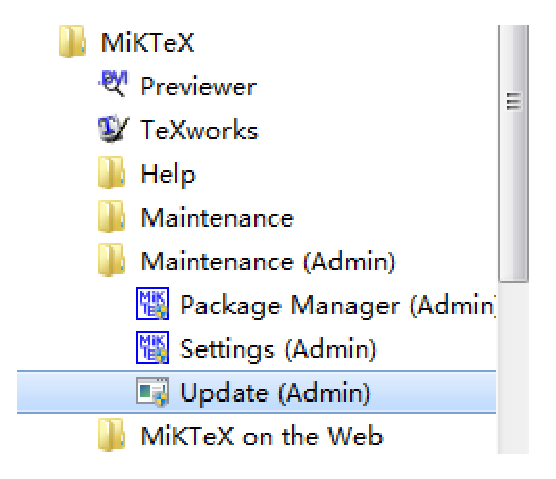
\includegraphics[scale=0.5]{./Pictures/set1.eps}\\
\caption{MiKTeX升级设置}
\label{set1}
\end{figure}

\begin{figure}[th]
\centering
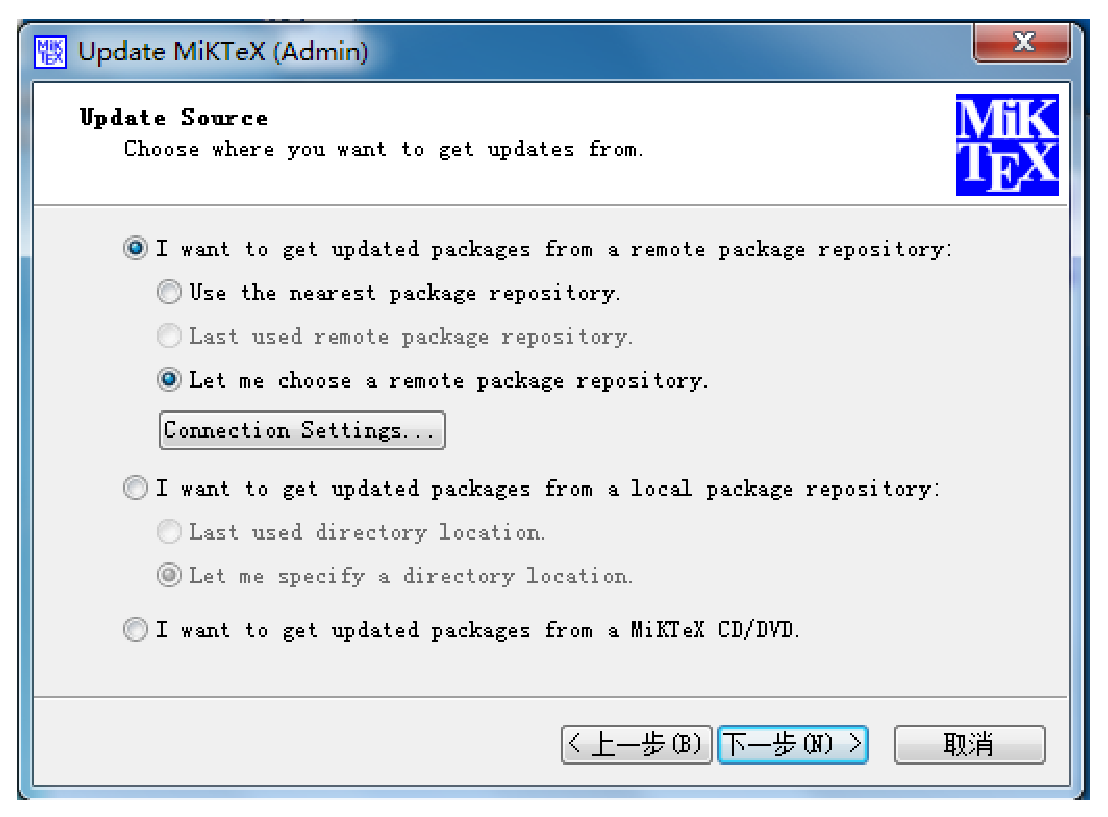
\includegraphics[scale=0.5]{./Pictures/set2.eps}\\
\caption{选择升级方式,如图中选择一个升级站点}
\label{set2}
\end{figure}

\begin{figure}[th]
\centering
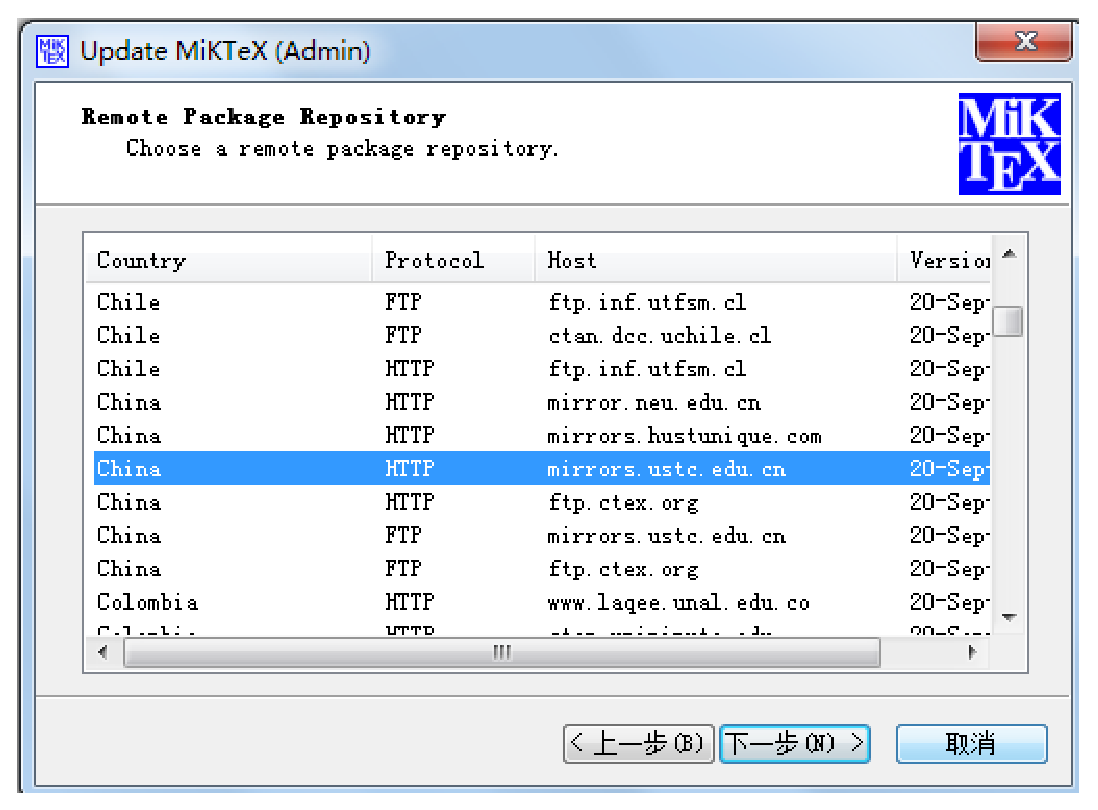
\includegraphics[scale=0.5]{./Pictures/set3.eps}\\
\caption{选择升级站点,以中科大镜像点为例}
\label{set3}
\end{figure}

之所以要把软件升级到最新是因为该模版使用了最新的hyperref包中添加的命令hidelinks。

\subsection{64位系统}

包括windows XP 64bit,Windows Server 2003 64bit,Vista 64bit,
Windows Server 2008 64bit,Windows 7 64bit 和 Windows Server 2008 R2。
当然现在还有了Windows 8,Windows 8.1和Windows 10。

安装CTeX安装包时,不要选择MiKTeX,其它软件任意,与32位一样。
安装完CTeX包后,去www.miktex.org网站下载MiKTeX的最新64位版,当前是2.9版,

安装后不需要进行特殊的设置,现在的CTeX功能包已经是latex扩展库中的一部分,
可以直接通过发行版自带的包管理系统下载安装该功能包。如图\ref{Roots}所示,在设置界面中的Root设置留空即可。

\begin{figure}[th]
	\centering
	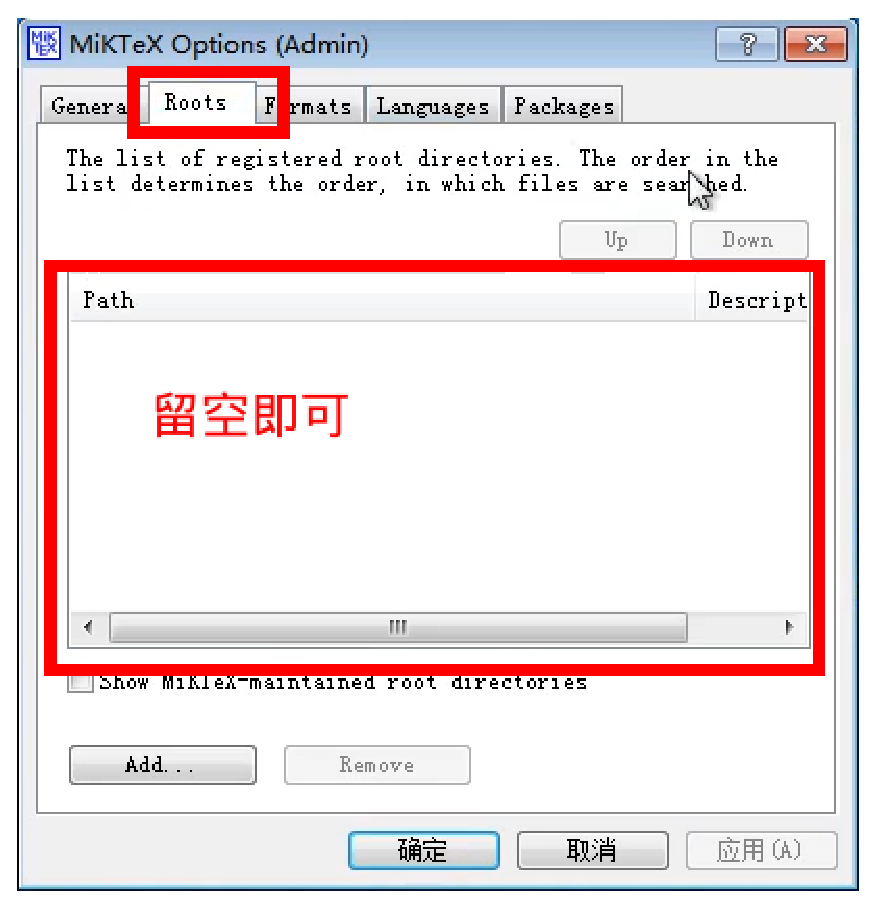
\includegraphics[scale=0.5]{./Pictures/Roots.eps}\\
	\caption{MiKTeX的Roots设置}
	\label{Roots}
\end{figure}

与32位Windows系统相同,安装完后也需要把MiKTeX升级到最新。

\section{linux系统}

请自行选择\LaTeX 安装版本,然后把CTeX环境加入即可。我想用linux的应该都会这个吧。
本次版本使用的操作系统及软件环境是ubuntu 14.04和TeXLive2014。

请保证扩展包版本足够新。尤其是hyperref包,保证是2011年8月份后的版本。

\section{Mac系统}

请自行选择\LaTeX 安装版本,加入CTeX环境。同linux下方法。一般是TeXLive,
通过其自带的包管理加载所需要的功能扩展包。

\section{本模版所需要的扩展包}

\begin{enumerate}

\item{图形、表格类扩展包} graphicx,array,booktabs,caption,natbib,multirow

\item{字体类扩展包} times(\LaTeX{}引擎中用),fontspec(\XeTeX{}引擎中用)

\item{目录选项扩展包} tocbibind,tocloft,makeidx,hyperref

\item{数学公式扩展包} amsmath,amsthm,amsfonts,amssymb,bm

\end{enumerate}

\section{测试运行}

如果已经安装好了CTeX环境与\LaTeX 软件,那么,可以运行这个模版文件包里的makethesis.bat文件,
几秒钟到十几秒后,如果生成了一份叫做“论文模版示例.pdf”的文档,那么,恭喜,这个模版所需要的软件环境建立成功!
如果没有生成这一份文件,那么有可能你的软件环境没有配置正确,比如把\LaTeX 软件升级到最新,
这份模版所需要的扩展包没有被安装,请打开\LaTeX 软件自动升级功能,
保证\LaTeX 软件能够成功地连接到CTAN站点下载所需的扩展功能包。

以Windows 系统gbk版本为例,具体测试运行过程如下:

打开cmd命令行工具,进入该模版所在目录,输入\LaTeX 命令如图\ref{runbat} 所示:

\begin{figure}[th]
	\centering
	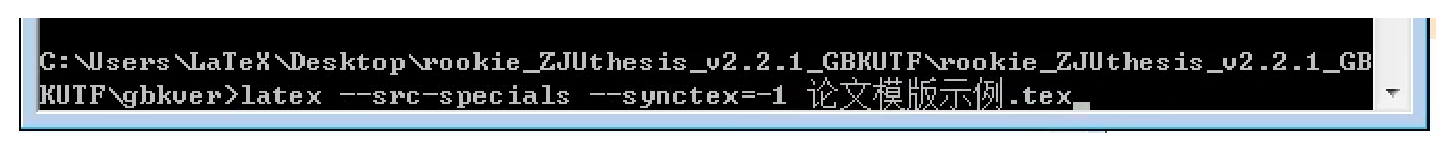
\includegraphics[scale=0.5]{./Pictures/runbat.eps}\\
	\caption{cmd窗口中运行\LaTeX 命令}
	\label{runbat}
\end{figure}

如果系统中MiKTeX的扩展包未安装完全,可能会弹出如图\ref{SelRep}所示窗口。
点“Change”按钮选择一个网络安装源。如果不选择就是由系统随机选择一个源(Random package repository)。

\begin{figure}[th]
	\centering
	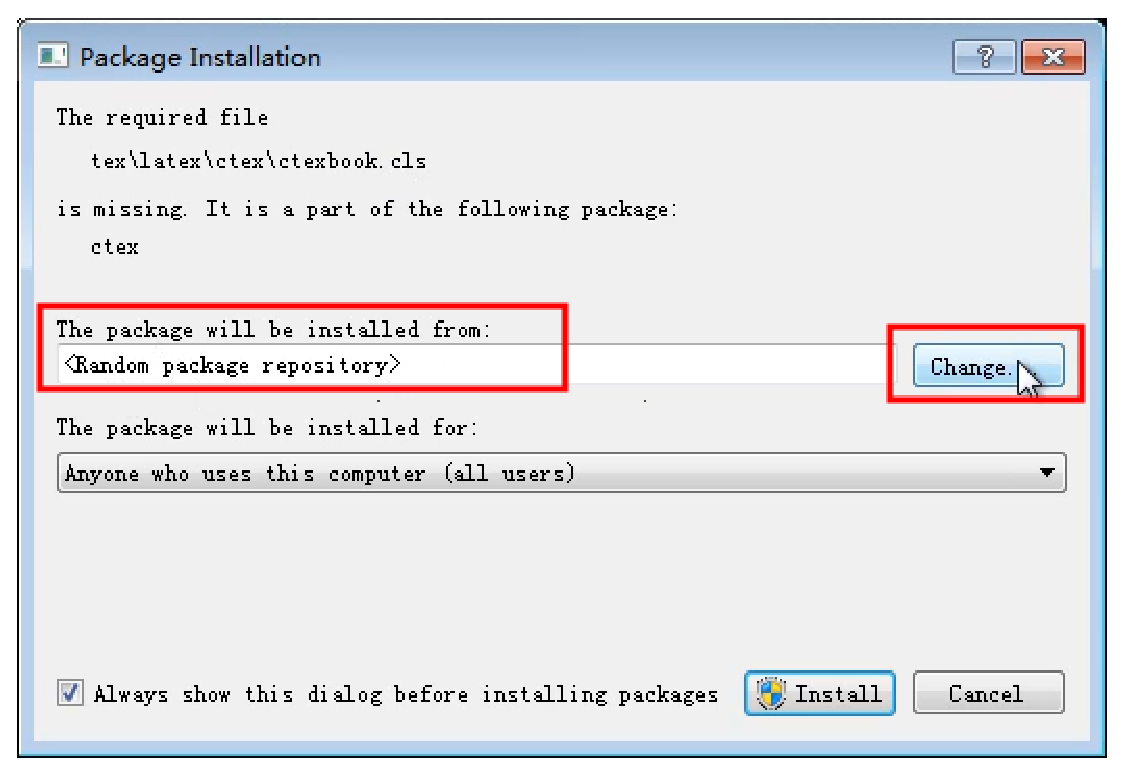
\includegraphics[scale=0.5]{./Pictures/SelRep.eps}\\
	\caption{下载缺少的扩展功能包}
	\label{SelRep}
\end{figure}

\newpage

点了"Change"按钮之后,在如图\ref{PkgInternet}所示界面中选择从网络源上下载。

\begin{figure}[th]
	\centering
	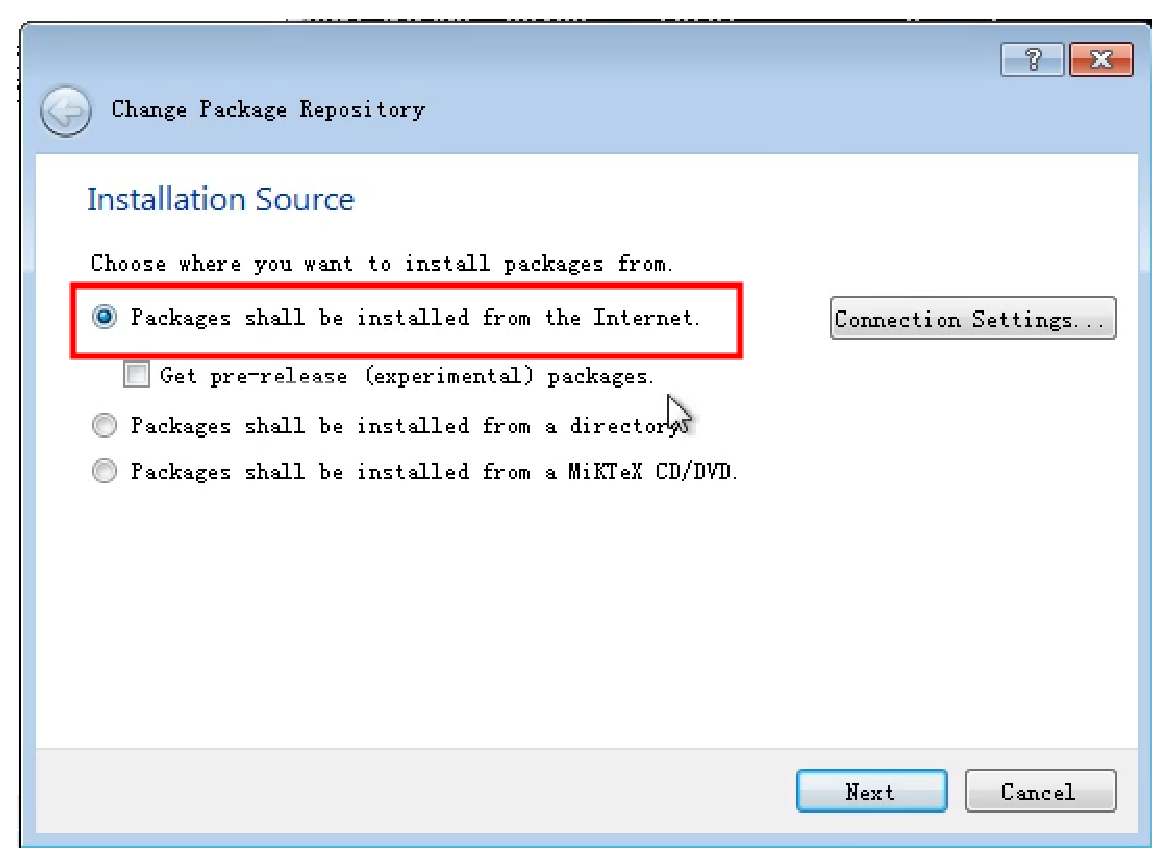
\includegraphics[scale=0.5]{./Pictures/PkgInternet.eps}\\
	\caption{选择网络源}
	\label{PkgInternet}
\end{figure}

下一步,选择一个源,最好是国内的源,速度比较快,如图\ref{SelRep_0}所示。
推荐使用HTTP协议,用FTP协议的站容易连接失败。

\begin{figure}[th]
	\centering
	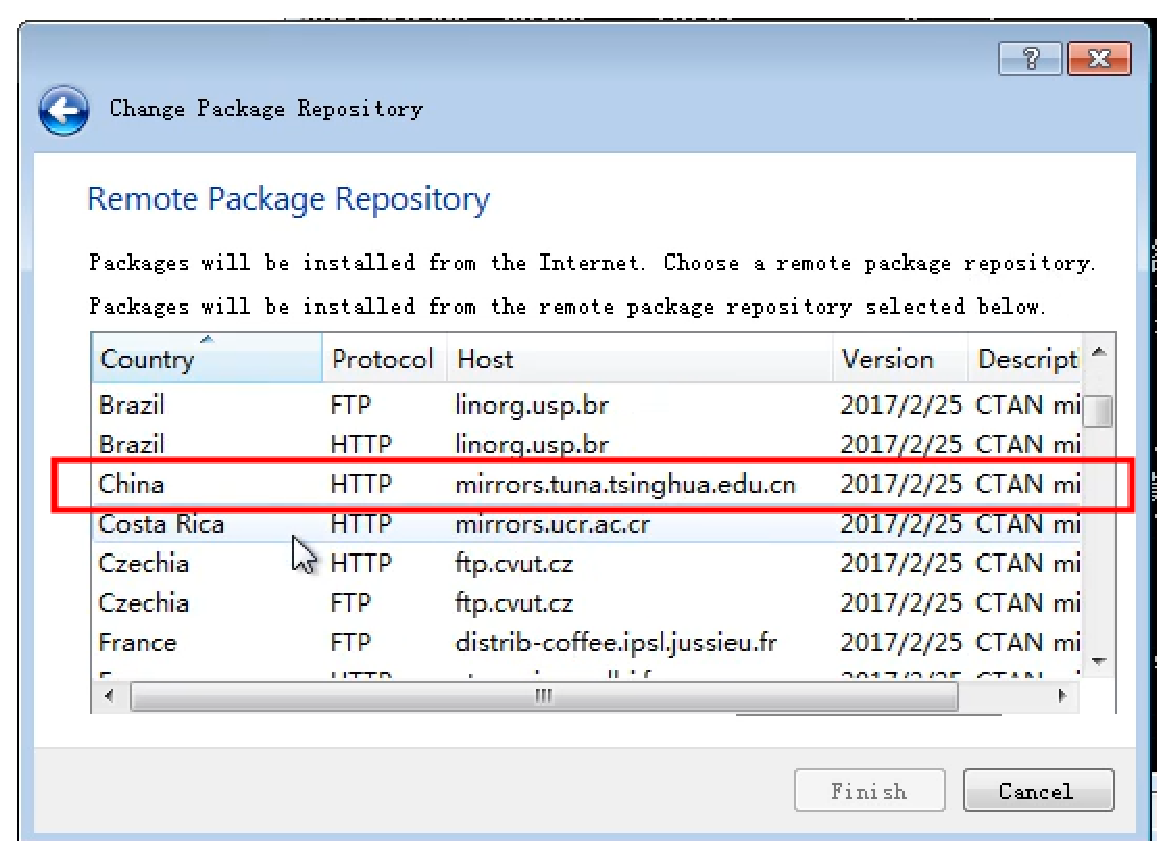
\includegraphics[scale=0.5]{./Pictures/SelRep_0.eps}\\
	\caption{选择国内安装源}
	\label{SelRep_0}
\end{figure}

\newpage

选择好之后,按“Install”按钮。如图\ref{PkgSelect}所示。

\begin{figure}[th]
	\centering
	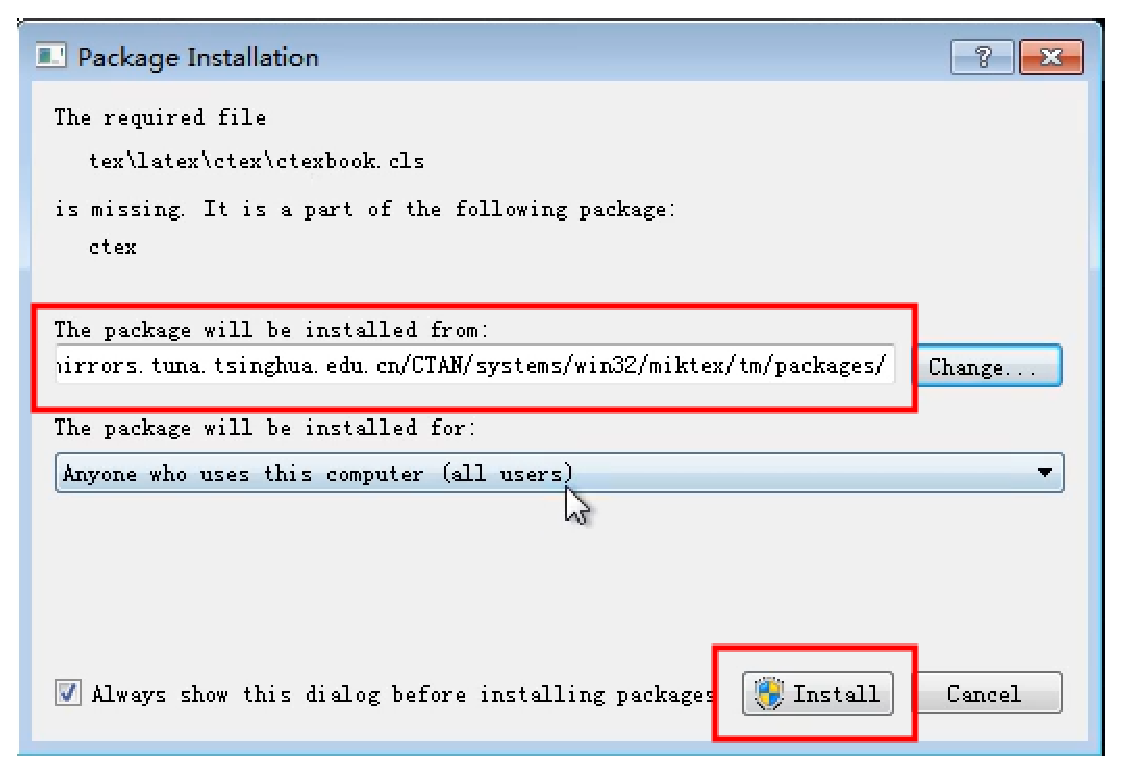
\includegraphics[scale=0.5]{./Pictures/PkgSelect.eps}\\
	\caption{选择好之后安装}
	\label{PkgSelect}
\end{figure}

按下安装之后,即可下载缺失包。如图\ref{Download}所示。

\begin{figure}[th]
	\centering
	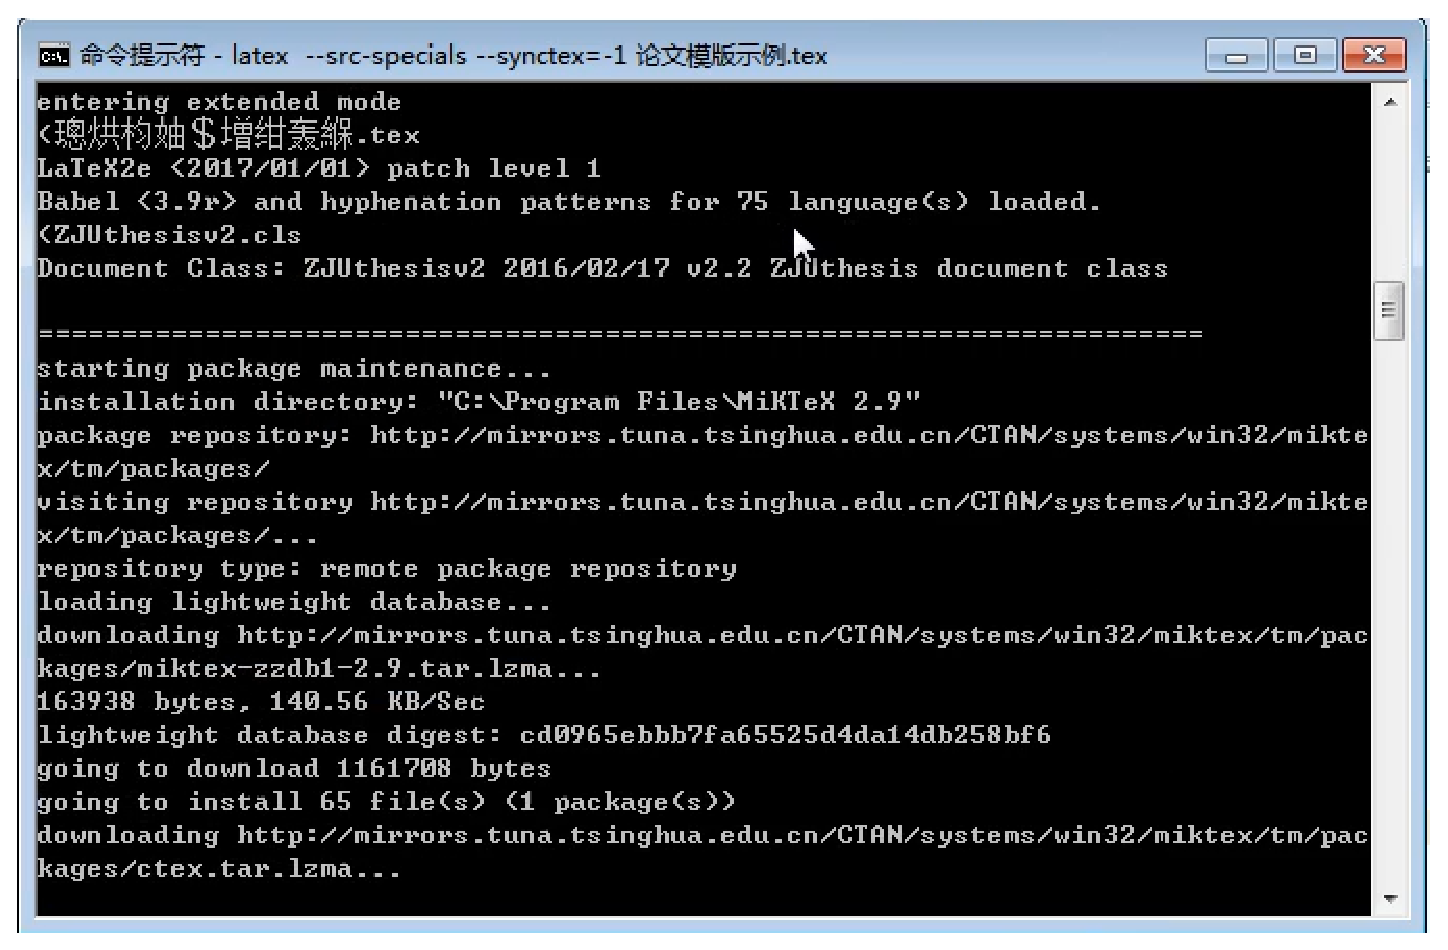
\includegraphics[scale=0.5]{./Pictures/Download.eps}\\
	\caption{选择好源后,下载过程中}
	\label{Download}
\end{figure}

\newpage

但这样每缺一个包,就会提示一次,这样会比较烦,可以把下面这个选择点掉,再按“Install”按键。

\begin{figure}[th]
	\centering
	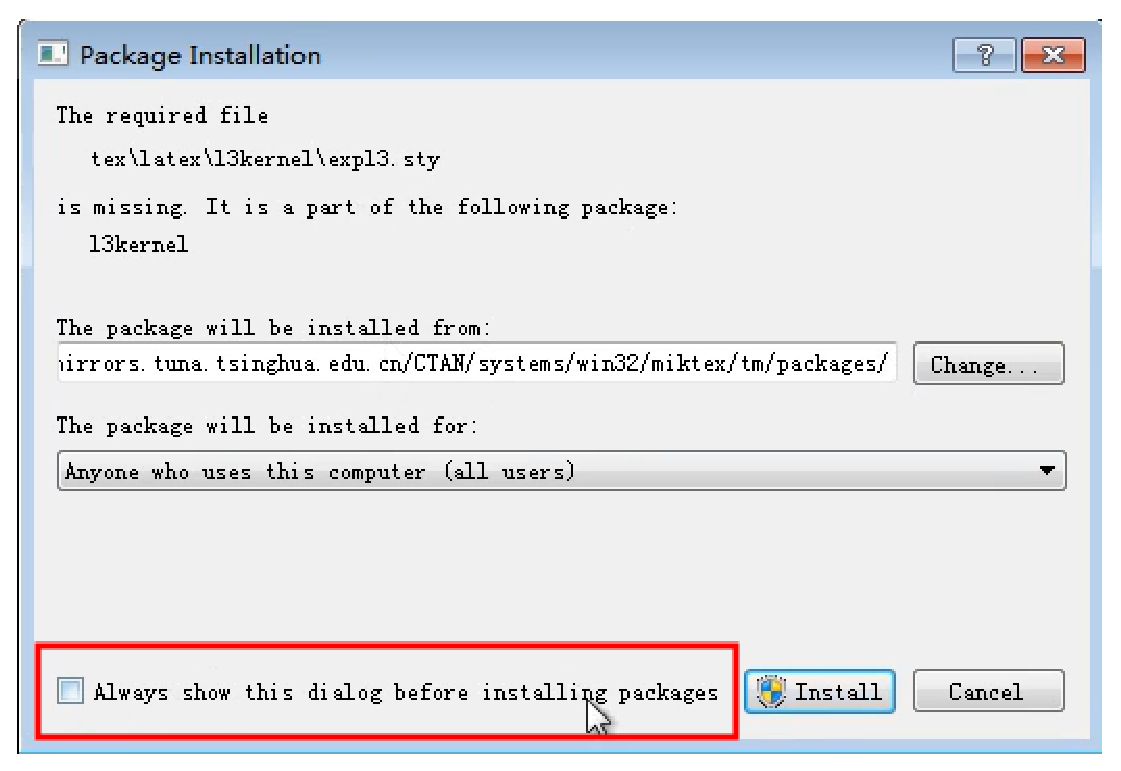
\includegraphics[scale=0.5]{./Pictures/NoShow.eps}\\
	\caption{点掉每次提示的选项}
	\label{NoShow}
\end{figure}

持续自动下载缺失的包如图\ref{l3kernel}所示。

\begin{figure}[th]
	\centering
	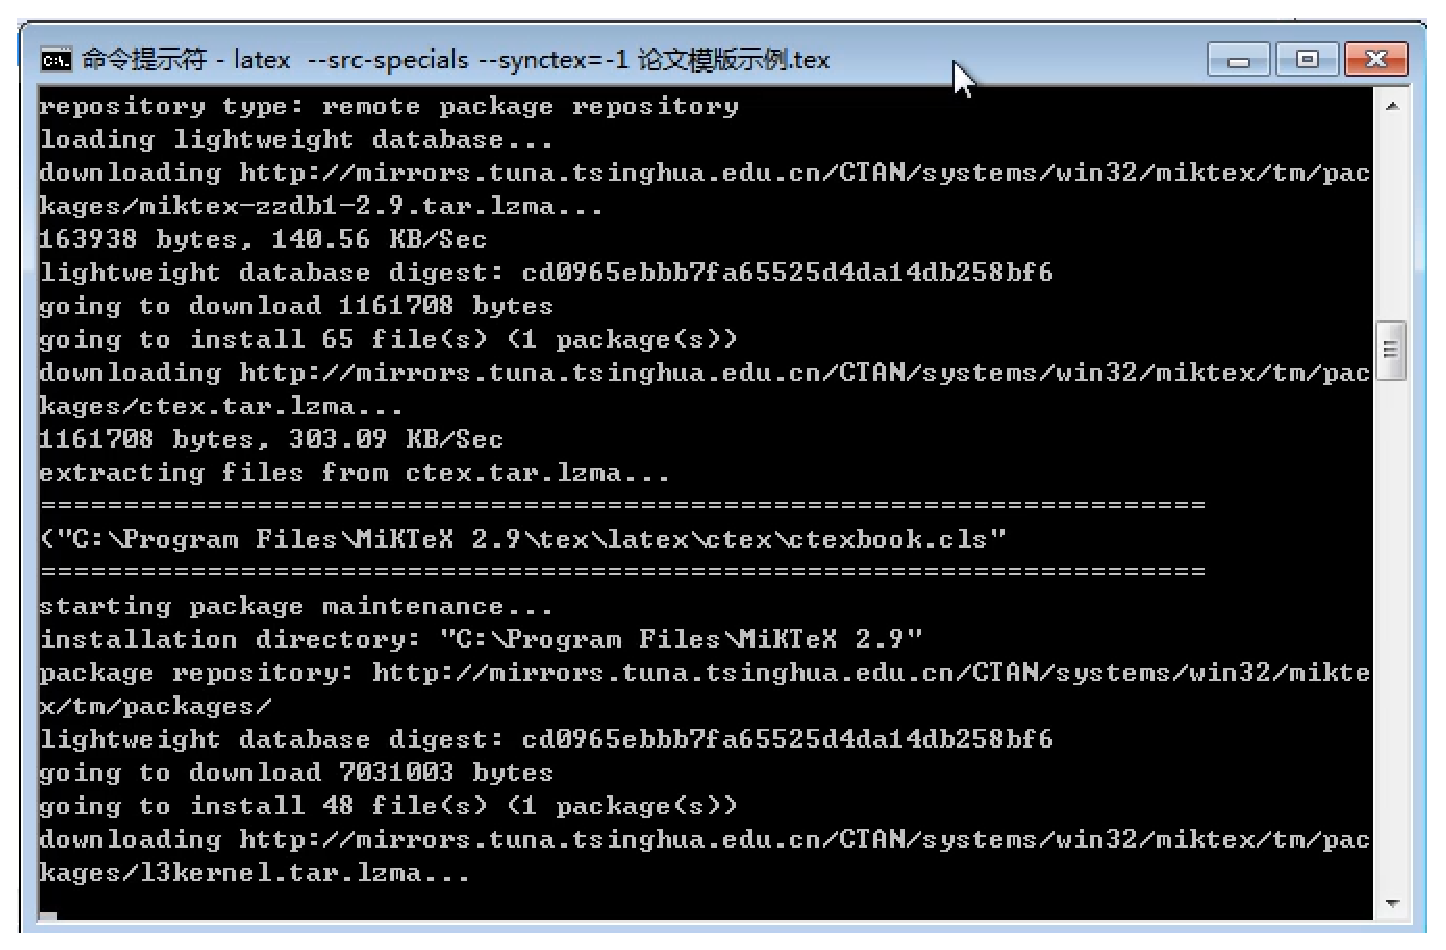
\includegraphics[scale=0.5]{./Pictures/l3kernel.eps}\\
	\caption{持续自动下载缺失的扩展包}
	\label{l3kernel}
\end{figure}

\newpage

\LaTeX 运行完成后,需要将生成的dvi转换为pdf,运行dvipdfmx进行转换。这个地方要提一点的是,
如果系统中字体没有安装完全, 比如隶书与幼圆字体没有安装,就会出现如图\ref{dvierror}所示的错误提示。

\begin{figure}[th]
	\centering
	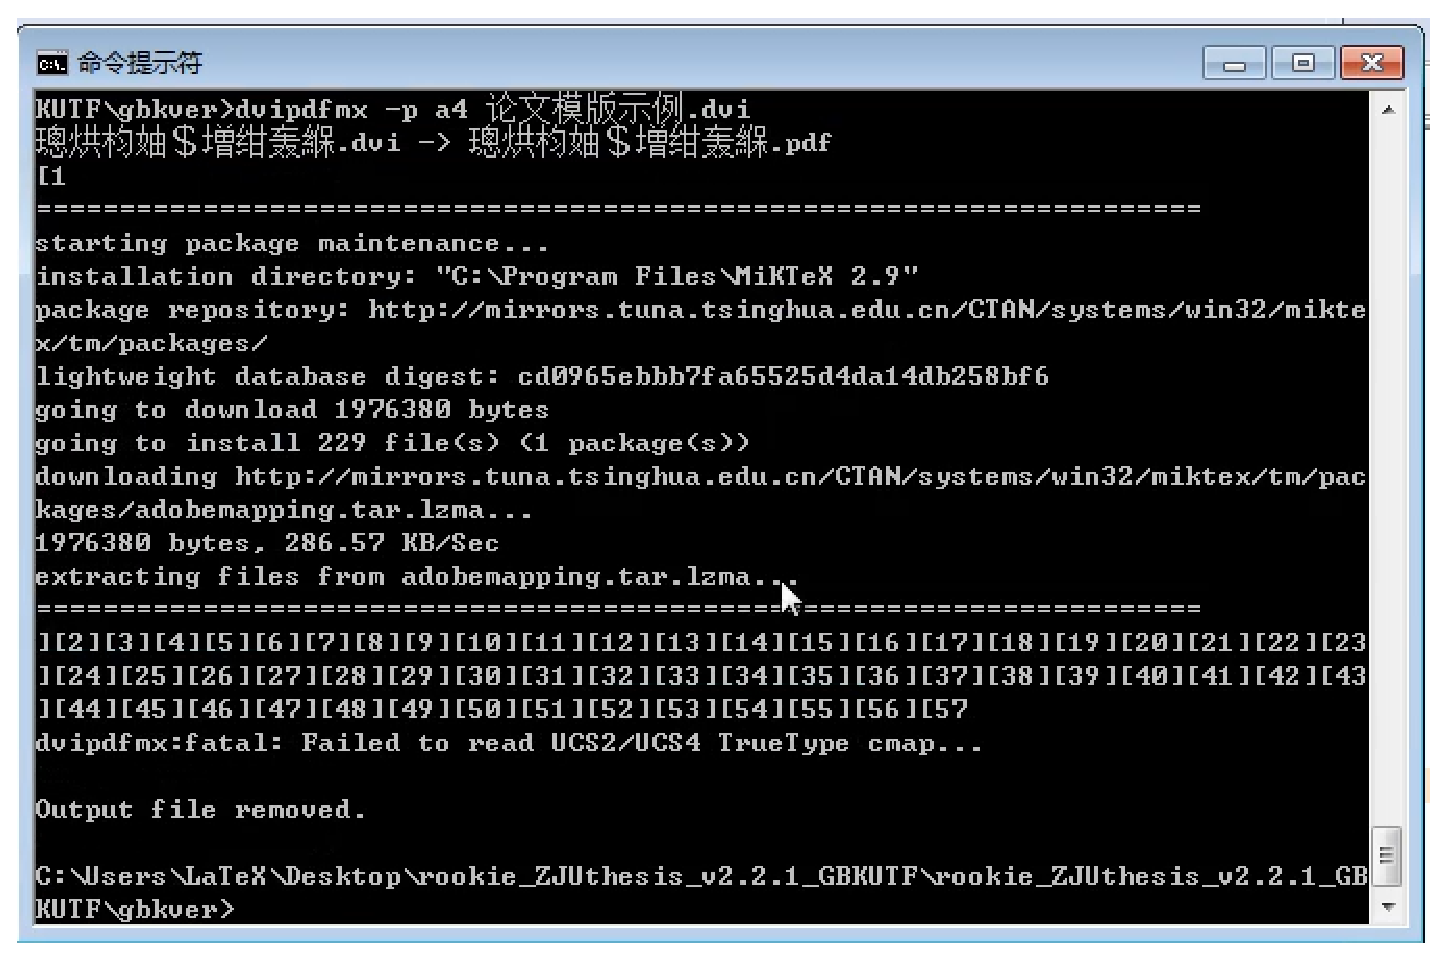
\includegraphics[scale=0.5]{./Pictures/dvierror.eps}\\
	\caption{转换pdf时可能出现的错误}
	\label{dvierror}
\end{figure}

将缺失的隶书与幼圆字体装入系统后,正常运行输出了pdf,如图所示。

\begin{figure}[th]
	\centering
	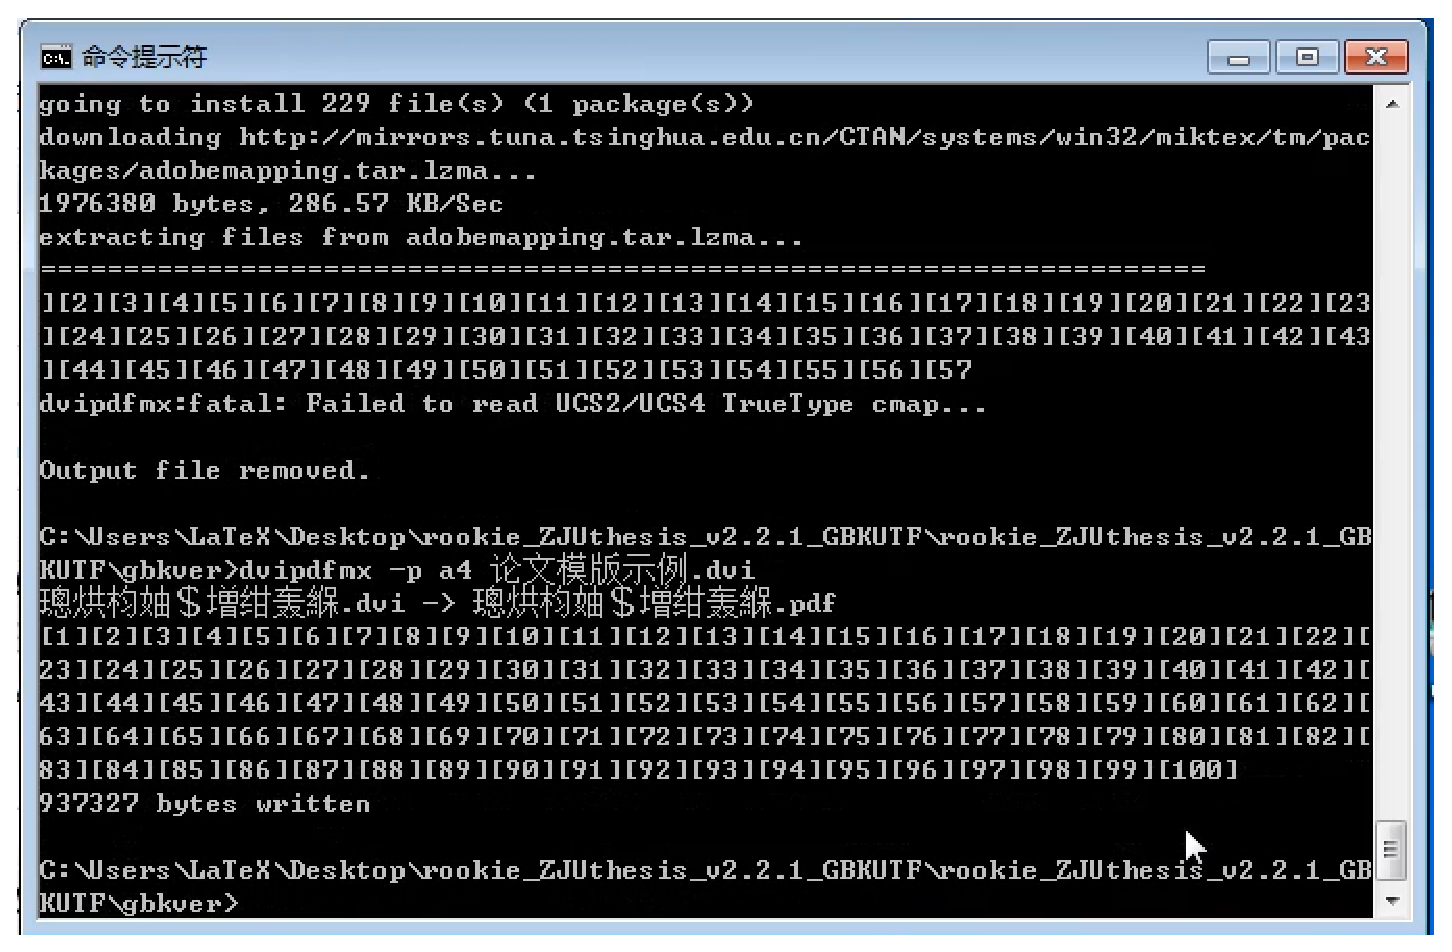
\includegraphics[scale=0.5]{./Pictures/complete.eps}\\
	\caption{生成pdf成功}
	\label{complete}
\end{figure}

使用\XeTeX 的utf版的使用过程与上述gbk版的过程类似,中间也会下载一些缺失的扩展包。

\chapter{使用该模版}

下面开始介绍如何使用这个模版,序言里已经提过,
这个模版的目的就是让没有一点\LaTeX 基础的同学也能很快地用\LaTeX 组织出自己的论文。
因此,这个模版没有过多的选项,只有一些和写Word同等难度\footnote{是的,难度少很多很多。这是一个测试用的脚注}的注意事项。
但难点,要比Word少很多。

这个模板一共需要如下几个文件:
\begin{enumerate}
\item{ZJUthesis.cls},这个是模版文件;
\item{ZJUthesis.cfg},这个是模版的配置文件,与模版文件配合使用;
\item{ZJUthesis.bst},这个是参考文献的格式说明文件;
\item{文件夹CoverPagepic},存放着封面使用到的浙大校名与校徽图片;
\item{CoverPagepic$\backslash$ZJDX.eps},eps\index{eps}格式\footnote{关于eps格式,
图片一节中将会做进一步介绍}的浙大校名图片;
\item{CoverPagepic$\backslash$ZJDX.pdf},pdf格式\footnote{同eps解释}的浙大校名图片;
\item{CoverPagepic$\backslash$QSY.eps},eps格式的校徽;
\item{CoverPagepic$\backslash$QSY.pdf},pdf格式的校徽。
\item{Chapter$\backslash$Copyright.tex},这个是版权转让声明。
\item{Signature$\backslash$sign\_ch.eps等七个签名文件},这个是作者签名,默认是一个空白的eps,提交最终版的时候可将其替换为相应的签名图片,直接可以作进pdf文档中去。这七个文件同样有其相对应的pdf格式图形文件,其文件名与相应签名对应如下:

{
\zihao{5}
\begin{tabular}{cl}
sign\_ch & 作者的中文签名(中文题名页用)\\
sign\_ch\_s & 导师的中文签名(中文题名页用)\\
sign\_en & 作者的英文签名(英文题名页用)\\
sign\_en\_s & 导师的英文签名(英文题名页用)\\
sign\_cr\_1 & 作者的中文签名(版权声明页用)\\
sign\_cr\_2 & 作者的中文签名(版权声明页用)\\
sign\_cr\_s & 导师的中文签名(版权声明页用)\\
\end{tabular}
}

当然,其中几个签名可以用同一个文件复制使用。也可以做七个不同的使用。
要注意的是签名的图形文件长宽比大约控制在2:1。
\end{enumerate}

现在即可以用winEdt或者其它习惯使用的文本编辑器,
打开这个文档的tex源文件,就是叫做“论文模版示例.tex”的这个文件。
我们书写论文,就是写这样一个扩展名为“tex”的纯文本文件。

我们现在开始它的第一行。

\section{模版选项}

%$\backslash$documentclass[oneside]\index{oneside}\{ZJUthesis\}
{\noindent\zihao{-5}\verb+\documentclass[oneside]{ZJUthesis}+}

这一句就指明了这个文档所用的格式模版,就是浙大的论文模版,{\bf ZJUthesis}
就是这个模版文件的文件名。
而{\bf$\backslash$documentclass}则是一个命令,在\LaTeX 源文件中,
以斜线$\backslash$开头的的字母字符串,都是一个命令,
命令只能由一个斜线及其引领的字符串构成,不能包含数字与其它符号,
当遇到非字母的其它字符时,该命令名字符串结束。因此,{\bf$\backslash$documentclass}
是一个命令,不包含其它内容。该命令的参数,就是被包含在
\{\}中的“ZJUthesis”,这个命令就是说明该文档使用的格式模版。而[oneside]则是{\bf ZJUthesis}
这个模版的参数。这个参数表示该论文现在采用单面印刷模式。

这个模版说明提供的可用选项只有两个\footnote{2.2.2版后UTF-8版增加一个选项AutoFakeBold=true,这个选项是为解决在Windows系统下,使用\XeTeX 时中文字体不能加粗的问题}:一个论文的单双面模式,另一个就是论文中链接的颜色。
其中论文的单面模式是通过在
$\backslash$documentclass[oneside]\{ZJUthesis\}中插入的[oneside]来实现的,
当把[oneside]换成[twoside]\index{twoside}或者删除时,论文就变成了双面模式。

你可以按上面说的把这个说明文档改成双面模式,然后保存,再运行makethesis.bat,生成出来的“论文模版示例.pdf”\footnote{生成新的“论文模版示例.pdf时,如果该文件正被打开,请先关闭。否则可能不会生成新的文件。”},看看跟单面模式有何不同?

你想让论文是单面还是双面?选择就是这样简单!

在tex源文件中,以\%起头的行都是注释行,在生成论文时,这些行将不会被论文包含,
所以,可以利用注释行来写一些你对你的论文中一些文字的评注,比如一段内容暂时不放进去,
不必删除它们,只需要把它们注释掉。就像这样:

{\zihao{-5}
\begin{verbatim}
% 这一段话我暂时先不放到论文里。
这一段话将出现在论文里。
\end{verbatim}
}
我们继续往下看:

这里我们看到了第二个参数,链接的颜色参数:

%$\backslash$hypersetup\{colorlinks=false\}
{\noindent\zihao{-5}\verb+\hypersetup{colorlinks=false}+}

简单来说,就是这个模版会给这份文档中的链接,比如目录,索引,参考文献的编号加上颜色,
以表示点击这个编号就能跳到相关的地方去。当然打印论文的时候我们并不想让它们有颜色,
这个选项就是这个目的,如果你把“false”改成了“true”,那么保存后,再运行一下makethesis.bat,
看一下生成的“论文模版示例.pdf”中目录跟之前有何不同。

再往下来就是文档的开始,用语句

%$\backslash$begin\{document\}
{\noindent\zihao{-5}\verb+\begin{document}+}

表示开始,


文档的最后有

%$\backslash$end\{document\}
{\noindent\zihao{-5}\verb+\end{document}+}

表示整个文档结束相呼应

接下来

%$\backslash$fangsong
{\noindent\zihao{-5}\verb+\fangsong+}

表示整个文档正文字体使用仿宋字体。
小四字号已经在模版中设置好了,此处无须设置。

\section{论文封面题名信息}

封面已经在模版中制作过,只需填入相应信息即可。

\vspace{8pt}

{\linespread{1}
\zihao{-5}\noindent
%$\backslash$classification\{TP311\} 
\begin{tabular}{p{5cm}p{10cm}}
\verb+\classification{TP311}+
&
\parbox[t]{10cm}{中图分类号,各专业分类号具体可以在 \\
http://grs.zju.edu.cn/News/html/grs/xwsqjgf/xwsq/xwsq\_{}bszn/2008-09-24/282-20080924085824.html 查询。}\\

%$\backslash$serialnumber\{10335\}
\verb+\serialnumber{10335}+
&
单位代码,浙大是10335。\\

%$\backslash$SecretLevel\{绝密\} 
\verb+\SecretLevel{绝密}+
&
保密级别,如果没有,就不写这一句,封面上就不会出现保密级别。\\

%$\backslash$PersonalID\{1234567\}
\verb+\PersonalID{1234567}+
&
申请号,一般是个人学号。\\

%$\backslash$title\{大家好,我是论文名\} 
\verb+\title{大家好,我是论文名}+
&
论文名。\\

%$\backslash$titletl\{上面一行写不下\}
\verb+\titletl{上在一行写不下}+
&
如果论文名太长一行写不下,则分两行写,这里写第二行题目。
如果一行就写得下,这一句不用出现。\\
\end{tabular}
}

\vspace{8pt}

如果论文名是两行,则请自行注意两行长度的分配。

\begin{center}
  \begin{tabular}{rl}
    {\bf\fangsong\zihao{-4}中文论文题目:} 
    &
    \bf\fangsong\zihao{5} \ZJUunderline[180pt]{我是第一行我比第二行长} \\[0mm]
    &
    \bf\fangsong\zihao{5} \ZJUunderline[180pt]{我是第二行我短} \\[0mm] 
  \end{tabular}
\end{center}

\begin{center}
  \begin{tabular}{rl}
    {\bf\fangsong\zihao{-4}中文论文题目:} 
    &
    \bf\fangsong\zihao{5} \ZJUunderline[180pt]{我是第一行我短} \\[0mm]
    &
    \bf\fangsong\zihao{5} \ZJUunderline[180pt]{我是第二行我比第一行长} \\[0mm] 
  \end{tabular}
\end{center}

这两种题目长度分配,请自行掌握。

\vspace{8pt}

{\linespread{1}
\zihao{-5}\noindent
\begin{tabular}{p{5cm}p{10cm}}
%$\backslash$englishtitle\{Thesis Title\}
\verb+\englishtitle{Thesis Title}+
&
论文英文名\\

%$\backslash$englishtitletl\{Second Line\}
\verb+\englishtitletl{Second Line}+
&
同样,如果论文名太长一行写不下,这里写第二行。
如果一行写得下,这一句也不用出现。\\

%$\backslash$Author\{大名在此\} 
\verb+\Author{大名在此}+
&
姓名,请填上自己的名字。\\
\end{tabular}
}

\vspace{8pt}

如果想让名字各个字之间有个间距,如下所示效果:

\begin{center}
  \begin{tabular}{l@{:}r}
    \zihao{-4}申请人姓名 & \fangsong\zihao{4}\ZJUunderline[160pt]{王\hspace{1.5em}东\hspace{1.5em}举}\\
  \end{tabular}
\end{center}

则在填写姓名的时候按如下格式填写:

%$\backslash$Author\{王$\backslash$hspace\{1.5em\}东$\backslash$hspace\{1.5em\}举\}
{\noindent\zihao{-5}
\verb+\Author{王\hspace{1.5em}东\hspace{1.5em}举}+}

其中的 $\backslash$hsapce\{{\bf1.5em}\} 表示空间间距为{\bfseries 一个半字符},
如果要{\bfseries 一个字符}间距,则写{\bf 1em}\footnote{$\backslash$hsapce\{1em\}也可以写作$\backslash$quad。},{\bfseries 两个字符}的间距,则是{\bf 2em},以此类推。

\vspace{8pt}

{\linespread{1}
\zihao{-5}\noindent
\begin{tabular}{p{8cm}p{7cm}}
%$\backslash$degree\{某士\} 
\verb+\degree{某士}+
&
什么学位的论文,填“硕士”或者“博士”。\\

%$\backslash$supervisor\{导师姓名$\backslash$hspace\{1em\}职称\}
\verb+\supervisor{导师姓名\space{1em}职称}+
&
填导师姓名与职称,
填法与自己姓名填法类似,如果姓名中间要插入空白,请参考自己姓名中空白的插入法。\\

%$\backslash$cpsupervisor\{合作导师姓名$\backslash$hspace\{1em\}职称\} 
\verb+\cpsupervisor{合作导师姓名\hspace{1em}职称}+
&
如果有合作导师,
使用这个命令,没有,就不写这个命令,封面上内容会自动进行调整出不出现合作导师字样。\\

%$\backslash$major\{电气工程\}
\verb+\major{电气工程}+
&
请填自己的专业名称,如字间增加空格,
请参照姓名空格增加方法。\\

%$\backslash$researchdm\{研究方向\} 
\verb+\researchdm{研究方向}+
&
请填自己的研究方向。\\

%$\backslash$institute\{电气工程学院\}
\verb+\institute{电气工程学院}+
&
请填自己的学院名称。\\

%$\backslash$submitdate\{2011年10月10日\}
\verb+\submitdate{2011年10月10日}+
&
这是论文提交日期,请自行填写。\\

%$\backslash$defenddate\{2011年11月1日\} 
\verb+\defenddate{2011年11月1日}+
&
这是答辩日期,请自行填写,交草稿时此项不填,
会自动留空。\\
\end{tabular}
}

\vspace{8pt}

到这里,封面内容填写完毕,可以使用生成封面的命令
%\begin{center}
%$\backslash$makeCoverPage
%\end{center}

{\noindent\zihao{-5}\verb+\CoverPagepic+}


来生成封面。

\section{实战:生成自己的论文第一页}

看了上面的介绍,那么你是不是已经跃跃欲试准备将自己的论文从第一页开始了?下面就开始着手吧。

首先,先准备一个文件夹放与论文相关的所有文件,比如命名成“我的毕业论文”。
然后,把“使用该模版”一节中提到的几个必须的文件都拷到“我的毕业论文”文件夹中去。
接着,使用WinEdt或者其它文本编辑软件在“我的毕业论文”文件夹中建立一个扩展名为tex的文件,
文件名自己取,我这里以“LATEX论文模版使用说明”为文件名。
最后,编辑“LATEX论文模版使用说明.tex”为如下内容,具体元素内容请自行填写:

\vspace{5mm}

{
\linespread{1}
\noindent\zihao{-5}
%$\backslash$documentclass\{ZJUthesis\}
%$\backslash$hypersetup\{colorlinks=false\}
%$\backslash$begin\{document\}
%$\backslash$classification\{TM863\}
%$\backslash$serialnumber\{10335\}
%$\backslash$SecretLevel\{绝密\}
%$\backslash$PersonalID\{1234567\}
%$\backslash$titel\{论文题目\}
%$\backslash$titletl\{论文题目第二行\}
%$\backslash$englishtitle\{English Title\}
%$\backslash$englishtitletl\{Second Line\}
%$\backslash$Author\{名字\}
%$\backslash$supervisor\{导师名字\}
%$\backslash$cpsupervisor\{合作导师名字\}
%$\backslash$major\{专业名称\}
%$\backslash$researchdm\{研究方向\}
%$\backslash$institute\{所属学院\}
%$\backslash$submitdate\{提交日期\}
%$\backslash$defenddate\{答辩日期\}
%$\backslash$makeCoverPage
%$\backslash$end\{document\}
\begin{verbatim}
\documentclass{ZJUthesis}
\hypersetup{colorlinks=false}
\begin{document}
\classification{TM863}
\serialnumber{10335}
\SecretLevel{绝密}
\PersonalID{1234567}
\titletitel{论文题目}
\titletl{论文题目第二行}
\englishtitle{English Title}
\englishtitletl{Second Line}
\Author{名字}
\supervisor{导师名字}
\cpsupervisor{合作导师名字}
\major{专业名称}
\researchdm{研究方向}
\institute{所属学院}
\submitdate{提交日期}
\defenddate{答辩日期}
\makeCoverPage
\end{document}
\end{verbatim}
}

以上内容可以直接从“论文模版示例.tex”中拷出来,建议保留其中的注释部分。
编写tex源文件中,建议尽可能多做注释,以方便后期修改。

另一个注意的地方是,最后一行一定要是 {\bf$\backslash$end\{document\}},
你可以把“论文模版示例.tex”拉到最下面,看看它的最后是不是就是这样一句。

\begin{figure}{thb}
\centering
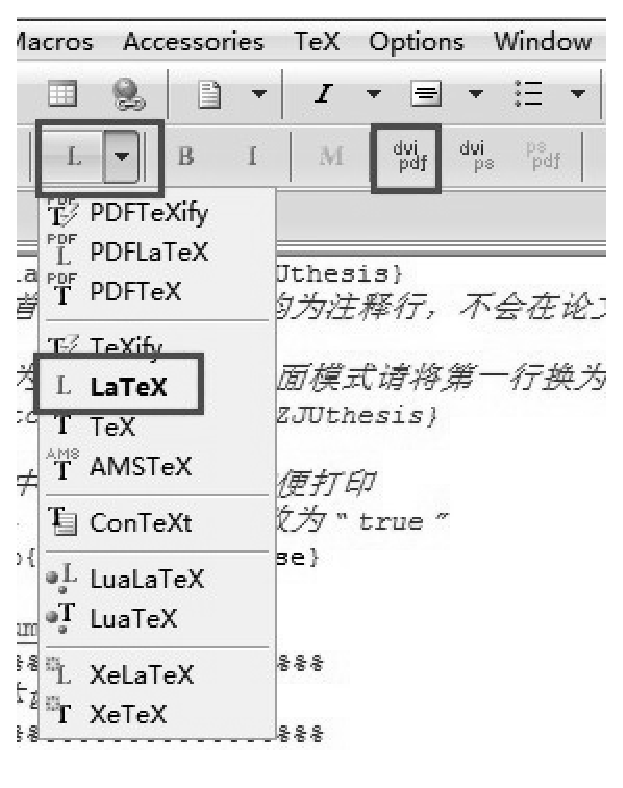
\includegraphics[scale=0.8]{./Pictures/runLaTeX.eps}
\caption{运行LaTeX}
\label{runLaTeX}
\end{figure}

然后点击WinEdt工具栏中的LaTeX命令,大约几秒运行完成后,
再点右边的dvipdf按钮,如图 \ref{runLaTeX} 所示,就可以生成
“LATEX论文模版使用说明.pdf”,打开就可以看到生成的封面了。

点“LaTeX”按钮的时候要注意的是,点右边的小箭头然后在下拉的菜单中只能是选中某个命令,此处选“LaTeX”,
要执行要点到按钮上才行。

还可以创建一个批处理文件来完成这个任务,此处批处理文件内容如下:

%\vspace{4mm}
{\linespread{1}
\zihao{-5}
\begin{verbatim}
latex --src-specials --synctex=-1 LATEX论文模版使用说明
dvipdfmx -p a4 LATEX论文模版使用说明
\end{verbatim}
}
\vspace{4mm}

当前目录下运行这个批处理命令也可以行到“LATEX论文模版使用说明.pdf”文件。

这里要说明的一点是,如果论文中开始加入参考文献,索引等信息,
那么生成pdf文档的流程还要增加,使用WinEdt操作顺序是:先点击“LaTeX”命令按钮,
再点击右边的“B”按钮(生成参考文献信息文件)和“I”按钮(生成索引信息文件);
然后{\bfseries 再}点击“LaTeX”命令{\bfseries 两次},最后再进行dvi到pdf的转换,
否则生成的pdf文件中参考文献与索引的引用处会是“?”号。
如使用批处理命令生成,则相应的批处理文件内容应修改如下:

%\vspace{4mm}
{\linespread{1}
\zihao{-5}
\begin{verbatim}
latex --src-specials --synctex=-1 LATEX论文模版使用说明
makeindex LATEX论文模版使用说明.idx
bibtex LATEX论文模版使用说明
latex --src-specials --synctex=-1 LATEX论文模版使用说明
latex --src-specials --synctex=-1 LATEX论文模版使用说明
dvipdfmx -p a4 LATEX论文模版使用说明
\end{verbatim}
}
\vspace{4mm}

\section{完成题名页信息}

从上节已经完成了封面的信息输入与创建,下面我们进入题名页的创建,
与创建封面页一样,题名页也是先输入信息,再创建页面。

还是回到“论文模版示例.tex”中,
题名页分中文题名页与英文题名页。
创建中文题名页要输入的信息有论文评阅人与答辩委员会名单,
当然,论文在草稿阶段这几个信息是不填的,待到答辩完成,
重新生成论文电子稿时,再填写这些信息。

论文评阅人信息代码及说明如下:

\vspace{8pt}
{
\linespread{1}
\zihao{-5}\noindent
\begin{tabular}{ll}
\verb+\reviewersA{姓\hspace{1em}名\hspace{1.5em}职称\hspace{1.5em}单位}+ & 论文评阅人1\\
\verb+\reviewersB{三字名\hspace{1.5em}职称\hspace{1.5em}单位}+ & 论文评阅人2\\
\verb+\reviewersC{三字名\hspace{1em}三字职\hspace{1em}单位}+ & 论文评阅人3\\
\verb+\reviewersD{姓\hspace{1em}名\hspace{1.5em}职称\hspace{1.5em}单位}+ & 论文评阅人4\\
\verb+\reviewersE{姓\hspace{1em}名\hspace{1.5em}职称\hspace{1.5em}单位}+ & 论文评阅人5\\
\end{tabular}
}
\vspace{8pt}

为了使这部分信息排版美观,这里要注意一点:

规划好“姓名”、“职称”、“单位”所占的空间,单位名称占用空间
尽量不要超过十二个字。
比如:

\begin{center}
\begin{tabular}{l@{:}r}
论文评阅人1
&
\ZJUunderline[220pt]{姓\hspace{1em}名\hspace{1.5em}职称\hspace{1.5em}这个单位名比较长长长}\\
论文评阅人2
&
\ZJUunderline[220pt]{三字名\hspace{1.5em}职称\hspace{1.5em}这个单位名短\hspace{4em}}\\
论文评阅人3
&
\ZJUunderline[220pt]{三字名\hspace{1em}副职称\hspace{1em}这个单位名不很长\hspace{2em}}\\
\end{tabular}
\end{center}

就要比

\begin{center}

\begin{tabular}{l@{:}r}
论文评阅人1
&
\ZJUunderline[220pt]{姓名\hspace{1em}职称\hspace{1em}这个单位名比较长长长}\\
论文评阅人2
&
\ZJUunderline[220pt]{三字名\hspace{1em}职称\hspace{1em}这个单位名短}\\
论文评阅人3
&
\ZJUunderline[220pt]{三字名\hspace{1em}副职称\hspace{1em}这个单位名不很长}\\
\end{tabular}
\end{center}

看起来要好得多。

前者的代码如下:
{\linespread{1}
\zihao{-5}
\begin{verbatim}
\reviewersA{姓\hspace{1em}名\hspace{1.5em}职称\hspace{1.5em}这个单位名比较长长长}
\reviewersB{三字名\hspace{1.5em}职称\hspace{1.5em}这个单位名短\hspace{4em}}
\reviewersC{三字名\hspace{1em}副职称\hspace{1em}这个单位名不和很长\hspace{2em}}
\end{verbatim}
}

注意$\backslash$space{Xem}的用法,一个em就是一个字宽。把所有单位名填充到同一长度,
最长的单位名是10个字,6个字的单位名就要补4个em,8个字的单位名补2个em。
请根据具体情况自行调整。

答辩委员会信息代码及说明如下:

\vspace{8pt}
{
\linespread{1}
\zihao{-5}\noindent
\begin{tabular}{ll}
\verb+\chairman{姓\hspace{1em}名\hspace{1.5em}职称\hspace{1.5em}单位}+ & 答辩委员会主席\\
\verb+\commissionerA{三字名\hspace{1.5em}职称\hspace{1.5em}单位}+ & 答辩委员会成员1\\
\verb+\commissionerB{三字名\hspace{1em}三字职\hspace{1em}单位}+ & 答辩委员会成员2\\
\verb+\commissionerC{姓\hspace{1em}名\hspace{1.5em}职称\hspace{1.5em}单位}+ & 答辩委员会成员3\\
\verb+\commissionerD{姓\hspace{1em}名\hspace{1.5em}职称\hspace{1.5em}单位}+ & 答辩委员会成员4\\
\verb+\commissionerE{姓\hspace{1em}名\hspace{1.5em}职称\hspace{1.5em}单位}+ & 答辩委员会成员5\\
\end{tabular}
}

\vspace{8pt}

答辩委员会信息同样规划好姓名,职称,单位信息,规划方法与评阅人相同。

生成中文题名页

\vspace{8pt}
\verb+\maketitle+
\vspace{8pt}

保存文件,生成PDF预览效果。

英文题名页信息输入与中文题名页类似。

此处英文题名需再输入一次,同样如果一行写不下写成两行。两行分配请自行处理。

{
\linespread{1}
\zihao{-5}\noindent
\begin{tabular}{p{7cm}l}
\verb+\Etitle{English Title}+ & 英文标题\\
\verb+\Etitletl{Second Line}+ & 如果一行写不下,这里写第二行\\
\end{tabular}
}

英文题名页的评阅人与答辩委员会信息及说明如下:

{
\linespread{1}
\zihao{-5}\noindent
\begin{tabular}{ll}
\verb+\EreviewersA{Name\hspace{1.5em}Professional Title\hspace{1.5em}Organization}+ & 论文评阅人1\\
\verb+\EreviewersB{Name\hspace{1.5em}Professional Title\hspace{1.5em}Organization}+ & 论文评阅人2\\
\verb+\EreviewersC{Name\hspace{1.5em}Professional Title\hspace{1.5em}Organization}+ & 论文评阅人3\\
\verb+\EreviewersD{Name\hspace{1.5em}Professional Title\hspace{1.5em}Organization}+ & 论文评阅人4\\
\verb+\EreviewersE{Name\hspace{1.5em}Professional Title\hspace{1.5em}Organization}+ & 论文评阅人5\\
\verb+\Echairman{Name\hspace{1.5em}Professional Title\hspace{1.5em}Organization}+ & 答辩委员会主席\\
\verb+\EcommissionerA{Name\hspace{1.5em}Professional Title\hspace{1.5em}Organization}+ & 答辩委员会成员1\\
\verb+\EcommissionerB{Name\hspace{1.5em}Professional Title\hspace{1.5em}Organization}+ & 答辩委员会成员2\\
\verb+\EcommissionerC{Name\hspace{1.5em}Professional Title\hspace{1.5em}Organization}+ & 答辩委员会成员3\\
\verb+\EcommissionerD{Name\hspace{1.5em}Professional Title\hspace{1.5em}Organization}+ & 答辩委员会成员4\\
\verb+\EcommissionerE{Name\hspace{1.5em}Professional Title\hspace{1.5em}Organization}+ & 答辩委员会成员5\\
\end{tabular}
}

同中文题名页类似,这里的人名,职称,单位信息尽量用简写,否则英文一行可能会写不下。
另外,它们之间的间距请自行设计掌握,与中文信息间距设计方式一致。

至此,英文题名页信息输入完毕。用英文题名页命令生成英文题名页

\vspace{8pt}
\verb+\makeEtitle+
\vspace{8pt}

这里{\bfseries 不要忘记}还有{\bfseries 版权信息页}

{
\zihao{5}
\begin{verbatim}
\SignautreDateA{2013}{10}{11}
\SignautreDateB{2013}{10}{11}
\SignautreDateC{2013}{10}{11}
\makeOSandCPRTpage
\end{verbatim}
}

这里的三个时间命令对应版权信息页中的签字日期信息,
在草稿及送审阶段,这几个命令可以不写。会自动把这几个位置留空。

\section{正文部分各章节的书写}

自此,论文的封面,题名页与版本信息页生成完毕,开始进入论文正文的书写阶段。
下面的内容将不再以命令为主,而是以自己的论文内容为主。

还是回到“论文模版示例”,在正文部分的开始,我们看到这样一个命令:

\verb+\ZJUfrontmatter+

这个命令的意思是开始论文的正文部分,将页码重置为大写罗马数字,并从I开始。


在谈各部分使用之前,写简单谈一下内容部分的书写。
\LaTeX 的文章内容书写没有什么特别的格式,直接书写即可。
但需要注意以下几点:

\begin{enumerate}
\item{\LaTeX 会忽略中文字符间的空格,也就是说:}

{
\linespread{1}
\zihao{-5}
\vspace{8pt}
\noindent\verb+大家好,我的中间没有空格。+\\
{\zihao{-4}和}\\
\verb+大 家 好, 我  的    中   间 没 有 空      格。+
\vspace{8pt}
}

最后输出的内容是一样的。都是:

大家好,我的中间没有空格。

这个“中文字符”包括中文的标点符号,即“。”,“,”等。

如果需要在中文单词间插入空格怎么办?只需要用“\~{}”来代替空格,就像这样:

{
\linespread{1}
\zihao{-5}
\vspace{8pt}
\noindent\verb+大~家~好,~我~的~中~间有很多的空~格。+
\vspace{8pt}
}

这样输出就是这样了:

大~家~好,~我~的~中~间有很多的空~格。

但在英文单词前后的空格,\LaTeX 会{\bfseries 保留一个}。

\item{断行与分段}

\LaTeX 中,{\bfseries 单独一个回车}也会像空格一样被忽略,空行作为分段的标志,
多个连续空行等效于一个空行。此外,还有一个断行命令,
“$\backslash$$\backslash$”,或者是“$\backslash$linebreak”,
这个命令的作用是直接换行但不分段,即新换的行前不空两格。比如

{
\linespread{1}
\zihao{-5}
\vspace{8pt}
我是第一行,\\
我还是第一行。

我是第一段,

我是第二段。

\begin{verbatim}
我是第一行,\\
我是第二行。
\end{verbatim}
\vspace{8pt}
}

出来就是这个效果:

\vspace{8pt}

\hspace{2em}我是第一行,
我还是第一行。

\hspace{2em}我是第一段,

\hspace{2em}我是第二段。

\hspace{2em}我是第一行,\\
我是第二行。

\vspace{8pt}

因此,在编写论文tex文件的时候,同一段落内可以任意换行,
比如写一句话就换一行,这样有利于自己写的时候思路更清晰。
只要不留空行,最后生成的文件都是一整段。

\item{中英文混合编辑时的一个问题及解决方案}

如果某一段文字是中英文字符混合,比如含有单词,
那么如果不做一点特殊处理,\LaTeX 在生成PDF时可能会出现某一行最后一个英文单词突出行外。
解决这个问题的办法就是在英文字符、单词的前面及后面加上空格符号。
当然,这样不太符合我们自己的写作习惯,一个个加起来也太费事。
没关系,\LaTeX 的中文先驱们已经替我们简化了这个问题。
CCT套件中有一个程序:cctspace.exe,只要运行如下格式的命令:

\verb+cctspace [输入文件名] [输出文件名]+

就可以执行这个空格插入操作,而无须手工一个一个添加。

这个程序在安装CTeX环境时已经被安装,可直接使用。使用linux的同学们,请自行在参考文献中的网站中下载源代码编译。

关于这个命令更多的功能选项说明,请参考张林波的《关于新版CCT的说明》\cite{NewCCT:2006}的4.2节部分内容,
很短的,只有一页,纯中文说明文档。


\item{其它的一些要注意的内容}

\LaTeX 中有部分特殊符号不可直接输入,如下:

\verb+#   $   %   ^   &   _   {   }   \+

输入它们要用以下的命令

\verb+\#   \$   \%   \^   \&    \_{}    \{    \}    $\backslash$+

\end{enumerate}

以上就是书写论文正文内容时的一些说明,更多常见问题,请参考《一份不太简短的\LaTeXe 介绍》\cite{LaTeXshzh}和《CTeX FAQ》。
这两个文档都可以在开始--菜单--程序--CTeX--help中找到。


以下将分章节介绍各部分书写时如何使用该模版。

\subsection{勘误页}

其实很少有论文有这样一个部分,但作为一个部分,还是将其做到了模版内。如果不需要,直接将其注释掉或者删除即可。

勘误页的调用命令为

{
\linespread{1}
\zihao{-5}\noindent
\begin{verbatim}
\begin{corrigenda}
这里就写你的勘误内容。
\end{corrigenda}
\end{verbatim}
}

有同学可能会发现,在“论文模版示例.tex”中这部分不是这么写的,我在接下来的致谢介绍中将解释原因。

\subsection{致谢}

致谢的调整命令与勘误页类似,为

{
\linespread{1}
\zihao{-5}\noindent
\begin{verbatim}
\begin{thanks}
这里就写你的致谢内容。
\end{thanks}
\end{verbatim}
}

但是看“论文模版示例.tex”中这一部分却只是简单写了一句:

\verb+\begin{thanks}
在我写这个文档的过程中,得到了网络上很多网贴的帮助,在此感谢baidu,Google,感谢
~CTeX 社区http://www.ctex.org,\LaTeX{}学习园地:http://blog.sina.com.cn/wangzhaoli11,
中科大~CTAN~镜像http://mirrors.ustc.edu.cn/CTAN/,水木社区\TeX{}版等网站、论坛,
其他一些较小的个人网站,论坛不再一一点名,在此一并感谢。
感谢浙江大学数学系提供的原始模版,感谢88\TeX{}版。
\end{thanks}
+

这里的$\backslash$input命令指输入另一个tex文件的内容到当前位置,
就是说\LaTeX 在编译这份tex源文件时读到这里,会去找这里指定的另一个tex文件,
并把它的内容全部复制到这个位置。

这样做的好处是实现了论文的模块化,可以把论文的不现章节写到不同的文件里去,
每个文件都不会太长,更容易查看与修改。在这里这个命令所指向的文件就是当前目录中Chapters目录下的
thanks.tex文件。同学们可以去看一下,这个thanks.tex文件中的内容,是不是就是
跟我上面写的例子是一样的。

要注意的是,这里面的目录名与文件名不能为中文,否则会出错\footnote{linux下的同学可无视这条}。

\subsection{序言}

使用方法同致谢,代码如下:

{
\linespread{1}
\zihao{-5}\noindent
\begin{verbatim}
\begin{preface}
这里就写你的序言的内容。
\end{preface}
\end{verbatim}
}

\subsection{摘要}

摘要的填写与致谢类似,只多了一个关键字命令$\backslash$keywords,具体如下:

{
\linespread{1}
\zihao{-5}\noindent
\begin{verbatim}
\begin{abstractC}
这里就写你的摘要的内容。

\keywords{关健字1,关键字2}
\end{abstractC}
\end{verbatim}
}

\subsection{英文摘要}

英文摘要的填法与中文摘要完全一样,只是都是用英文,具体如下:

{
\linespread{1}
\zihao{-5}\noindent
\begin{verbatim}
\begin{abstractE}
这里就写你的摘要的内容。

\keywordsE{keywords1,keywords2}
\end{abstractC}
\end{verbatim}
}

这个地方要注意的是与中文摘要命令不同之处,abstractE与keywordsE。

\subsection{图片目录}

这一部分只需要如下一个命令,其它的东西\LaTeX 自己会替你搞定。

\verb+\ZJUListofFigures+

如果你不需要图片目录,那么把这条命令删去或者注释掉。

\subsection{表格目录}

这一部分同样只需要如下一个命令,其它的东西\LaTeX 会替你做好。

\verb+\ZJUListofTables+

如果你不需要表格目录,同样只要把这条命令删去或者注释掉即可。

\subsection{缩写、符号清单、术语表}

这一部分与致谢部分相似。代码如下:

{
\linespread{1}
\zihao{-5}\noindent
\begin{verbatim}
\begin{ListofSymbol}
这里就写你的缩写、符号清单、术语表的内容。
\end{ListofSymbol}
\end{verbatim}
}

\subsection{目录}

这一部分只需要如下一个命令,\LaTeX 会替你搞定一切。

\verb+\ZJUcontents+

\subsection{正文章节内容}

到这里,就到了正文章节的编写了。正文部分写法跟致谢,序言的相同,
但致谢,序言没有更小的分节,也不会有图片,表格等内容。
图片,表格方面内容在本说明中放在下面几章中,这里先只介绍正文的章节排布。

在开始正文内容之前,需要一个\LaTeX 命令来告诉软件进入正文部分,
页码需要重新从1编号,并使用阿拉伯数字,以及章节开始从1开始。这个命令是

\verb+\ZJUmainmatter+

正文会有很多章,概述,条件,分析,讨论,结论什么的。编写tex文件的时候,
需要给\LaTeX 明确哪些是章,哪些是节,哪一些是更小的节。这样,\LaTeX 才能正确地给你的正文内容分章,分节

章节标题命令及使用如下:

{
\linespread{1}
\zihao{-5}\noindent
\begin{verbatim}
\chapter{我是章的标题}
我是章标题下的内容
\section{我是第一节的标题}
我是节标题下的内容
\subsection{我是小节的标题}
我是小节的内容。
\begin{enumerate}
\item{我是并列项1}
\item{我是并列项2}
\end{enumerate}
\subsection{我是第二小节的标题}
我是第二小节的内容。
\section{我是第二节的标题}
我是第二节的内容
\subsection{我是第二节第一小节的标题}
我是第二节第一小节的内容
…………
\end{verbatim}
}

章节标题中不需要说明是第几章第几节,\LaTeX 会替你计算,
你所要做的只是把你的文章按结构统一起来即可。
并且,目次也会根据你的标题内容自动生成。
这里要补充一点的是:有的标题可能会比较长,写到目录里会导致目录条目换行,
为解决这个问题,\LaTeX 允许目录中的标题与实际的标题不一样,要达到这个效果,
以章的标题为例,其命令应加一个参数,如下:

\verb+\section[目录中的标题]{实际章节中的标题}+

该模版中章节加上段落可以有6层,足够用了。如表 \ref{ChapsecList} 所示。

\begin{table}[thb]
\zihao{5}
\caption{章节命令}
\label{ChapsecList}
\centering
\begin{minipage}[c]{9cm}
\centering
\begin{tabular}{p{6cm}|c}
\hline
命令 & 层次\\
\hline
\verb+\chapter+ & 章\footnote{实际上在章的上层还有一层叫做part(部分),本模版中用不到。}\\
\hline
\verb+\section+ & 节\\
\hline
\verb+\subsection+ & 小节\\
\hline
\verb+\subsubsection+ & 小小节\\
\hline
\verb+\paragraph+ & 段\\
\hline
\verb+\subparagraph+ & 分段\\
\hline
\end{tabular}
\end{minipage}
\end{table}

另外,如果某处需要用到几个并列项,可以采用enumberate命令,具体代码如下:
{
\linespread{1}
\zihao{-5}\noindent
\begin{verbatim}
  \begin{enumerate}

  \item{我是并列项1} 

  我是并列项1的内容。

  下面将有一个嵌套应用

  \begin{enumerate}
    \item{我是并列项1中的又一个并列项1}

    我是小并列项1的内容。

    \item{我是并列项2中的又一个并列项2}

    我是小并形项2的内容。
  \end{enumerate}

  \item{我是并列项2}

  我是并列项2的内容。

  \end{enumerate}
\end{verbatim}
}

生成文档的效果如下:

\begin{enumerate}
\item{我是并列项1}

我是并列项1的内容。

下面将有一个嵌套应用

\begin{enumerate}
\item{我是并列项1中的又一个并列项1}

我是小并列项1的内容。

\item{我是并列项2中的又一个并列项2}

我是小并形项2的内容。

\end{enumerate}
\item{我是并列项2}

我是并列项2的内容。

\end{enumerate}

\vspace{8pt}

注意tex代码部分中的空行。

这种并列项同样不需要考虑编号问题,\LaTeX 会替你做好一切。
嵌套应用最多可以嵌套三层。

\subsection{参考文献}

正文自此完成了,下面的内容是后面的参考文献,索引,简历等部分。
先需要一个命令告诉软件正文部分结束,开始文后部分

\verb+\ZJUbackmatter+

当正文部分完成后,下一个部分就是参考文献。
参考文献的生成需要准备另外一个参考文献数据文件*.bib,
本说明附带了一个数据文件例子:thesis.bib,
该文件也是一个纯文本文件,可以用记事本打开。
里面给出了七种参考文献的格式:
专利(patent)、标准(standard)、电子文档(Edoc)、
期刊论文(article)、书籍(book)、博/硕士学位论文(mastersthesis/phdthesis)、
其它文献(misc)。

下面以期刊论文为例来说明它的格式。

{
\linespread{1}
\zihao{-5}\noindent
\begin{verbatim}
@article{
LUOZ:2007,
   Author = {罗振 and 田丰 and 孙小平 and 孙恩岩},
   Title = {基于{LATEX}的学位论文模板的设计与实现},
   Journal = {沈阳航空工业学院学报},
   Volume = {24},
   Number = {3},
   Pages = {45-48},
   Year = {2007},
   lang = {chinese}}
\end{verbatim}
}

下面来逐行解释它们表示意义:

@article表示这个文献信息所代表的文献类型是期刊文献。
其它的文献类型见前两段内容。
它后面紧跟的大括号\{\}将这个期刊文献的所有信息括起来。

第二行的“LUOZ:2007”是这个参考文献的引用名,
可以起成任意的方便标识的字符组合,但不能使用中文。
这个字符组合将在文中引用时使用。
以这篇为例,当在论文中使用\verb+\cite{LUOZ:2007}+时,
在生成的文档中此处就会出现引用标号,具体标号\LaTeX 会自己去计算,
后面参考文献部分中的参考文献也由\LaTeX 去排列。
本模版设定的论文引用编号规则是按引用先后排序。

第三行到最后,每一行都代表了该文献的一项信息,
分别是:作者(Author),题目(Title),期刊(Journal),
卷号(Volume),期号(Number),页码(Pages),年份(Year),
语言(lang),每项信息都被\{\}括了起来。要{\bfseries 注意}除了最后一项,
每一项都以一个英文逗号“,”结束;多个作者之间用“and”连接;
如果题目中有连续的大写字母,应用\{\}把它们单独括起来,
如不括起来,除首单词首字母,其它都会被变回小写。

语言的信息项可以不写,这里写上是为了保障对中文文献信息的兼容。

其它几类文献的信息可参考thesis.bib中的填写方法,
与上述说明大同小异。

当所有参考文献信息按thesis.bib中格式填写好,存为一个*.bib文件,
文件名可以任意取,但不能使用中文,比如mybib.bib。

在tex源文件中,只需在文中按上面介绍的$\backslash$cite命令把引用
参考文献的地方一一用标识词标示出来,再在正文的最后使用如下所示的参考文献列表命令,
就可以生成格式完全符合要求的参考文献列表,
这个格式符合要求包括任何一个标点都是正确的!!

\verb+\ZJUthesisbib{mybib}+

请注意这里命令的参数就是你的参数文献数据文件的文件名。


\subsection{附录}

附录以命令\verb+\appendix+开始,随后即可写入附录章节内容。
附录章节内容写法与正文写法完全相同,\LaTeX 会替你处理好章节编号等问题,
你完全不用考虑附录的编号。

{
\linespread{1}
\zihao{-5}\noindent
\begin{verbatim}
\chapter{附录A}
\chapter{附录B}
\end{verbatim}
}

\subsection{索引}

索引与参考文献的使用方法类似,但不需要建立什么数据文件,只要你在文中有索引标记,
到了这里,只需要如下一条命令就能够建立索引。

\verb+\ZJUindex+


\subsection{个人简历}

个人简历部分比较简单,按如下格式书写即可。相信写完论文后,这个完全难不住你们的。

{
\linespread{1}
\zihao{-5}\noindent
\begin{verbatim}
\begin{resume}
\begin{enumerate}
\item{第一条的内容}
\item{第二条内容}
\end{enumerate}
\end{resume}
\end{verbatim}
}

\subsection{发表文章目录}

发表文章目录部分同个人简历部分,命令只是关键字不同。

{
\linespread{1}
\zihao{-5}\noindent
\begin{verbatim}
\begin{publications}
\begin{enumerate}
\item{第一篇}
\item{第二篇}
\end{enumerate}
\end{publications}
\end{verbatim}
}




\section{插入图片}

论文中会插入图片\index{图片}、表格\index{表格}等元素。在Word中插图也是一件比较头疼的事,
涉及图的位置布置,大小,清晰度等问题。在\LaTeX 中这些问题也在一定程度上存在,
但\LaTeX 尽可能使得排版出来效果较好。相对于Word,虽然不是所见所得形式,
初期学习比较繁琐,但经短时间熟悉后可以比Word处理快不少。
我最喜欢的方式就是用Octave+gunplot把曲线图做成标准一样的大小,然后把这些图命好名,
放到一个专门的目录中去,一次全插好,如果要修改所有图的大小及式样,只要修改一下相应的Octave的生成曲线脚本文件即可。
这样整篇文档中的曲线图都是统一的模式,统一大小,统一字体,非常整齐。

下面对\LaTeX 中常见的插入图片方法作简要介绍,对于大部分专业做毕业论文应该是足够了,
更多更复杂的方式,有兴趣的可以查找相关专题说明文档\cite{epslatex},
这里提到的文献[\citenum{epslatex}]中给的是英文原版的下载地址,中文版搜一下网上到处有。

\LaTeX 支持的图片格式分两种情况:

\begin{enumerate}

\item{tex-$>$dvi-$>$pdf方式}

包括tex-$>$dvi-$>$ps-$>$pdf这样一个过程,本模版推荐采用的方式是tex-$>$dvi-$>$pdf,
这样的处理流程下,只能采用eps\index{eps}格式的图片。
如果你只有jpg\index{jpg},jpeg,png,gif之类格式的图片,那么不要紧,
\LaTeX 中提供了一个转换程序bmeps.exe\index{bmeps},可以帮助你把jpeg图片转换成eps格式,
当然你也可以用photoshop\index{photoshop},gimp转换。使用bmeps的命令格式如下:

bmeps -p 1 -c picture.jpeg picture.eps

其中,-p 1是压缩出的图片质量,1最好,2是默认,3最差。-c是保留彩色,不带c图片为黑白。

\item{tex-$>$pdf方式}

如果是用pdfTeX\index{pdfTeX}直接将tex转换为pdf的流程,则不能采用eps格式,但可以采用jpg,jpeg,
png,gif这些格式。

如果只有eps格式图片,则可以使用photoshop,gimp或者Acrobat\index{Acrobat}将其转为pdf格式。

这也是为什么这个模版带的文件中既有eps又有pdf的原因,
为了照顾到部分直接将tex转换到pdf的同学。

\end{enumerate}

{\bfseries 本模版推荐新手使用eps格式图片。}
eps格式没使用过\LaTeX 可能会比较陌生,eps也是一种矢量格式\index{矢量}图形。就是说如果是从矢量图形
转到eps格式,一样可以无损缩放。

subsection{图片插入的一般方法}

在文中插入图片的常用命令如下(以使用eps格式为例):

{
\linespread{1}
\zihao{-5}\noindent
\begin{verbatim}
\begin{figure}[htb]
\centering
\includegraphics{picture.eps}
\caption{图片标题}
\label{Figflag}
\end{figure}
\end{verbatim}
}

\verb+\begin{figure}[htb]+是告诉\LaTeX 软件准备插入图片,[htb]是一个选项,
代表图片的插入位置,h代表在文中当前位置,t代表一页的顶部,b代表页面底部,
还有一个选项是p,代表图片要单独放在一页中,如果不给出这些选项,
\LaTeX 会试着依次选用h-t-b-p方式,找出自已认为最合适的,如果给出一选项,
\LaTeX 就只使用给出的一个选项,如果给出几个选项,\LaTeX 会尝试给出的这几个选项,
然后选用它认为最合适的。
一般采用默认方式,不给出任何选项。除非有个把图\LaTeX 自动给出的位置不好,
再通过这几个选项来选择。

\verb+\centering+表示图片的位置为居中放置。

\verb+\includegraphics{picture.eps}+指出了要添加的图片的文件名,
如果图片在其它目录中,比如pictures文件夹,命令则变为:\\
\verb+\includegraphics{pictures/picture.eps}+。\\
要着重说明的是,插入的图片可以采用选项进行缩放\index{缩放},旋转。
比如,要把图片设置为同文字部分一样宽,如图 \ref{FigTextWidth} ,
则命令变为:\\
\verb+\includegraphics[width=\textwidth]{picture.eps}+

\begin{figure}[htb]
\centering

\includegraphics[width=\textwidth]{./Pictures/LHS.eps}
\caption{跟文字一样宽的图}
\label{FigTextWidth}
\end{figure}

指定为与文字一样宽太宽了,下面来把它缩小点,比如半个文字宽度,
那么就用\verb+width=0.5\textwidth+,如果指定10cm宽,就用width=10cm,
如果指定7cm高,就用height=7cm,如果是指定原图大小的50\%,就用
scale=0.5,如果我们想把它调整到原尺寸大小的50\%,再逆时针旋转90度
(如想顺时针旋转则使用负角度值),
就用如下的命令:\\
\verb+\includegraphics[scale=0.5,angle=90]{picture.eps}+\\
效果如图 \ref{FigHalfr90} 所示。

\begin{figure}[htb]
\centering

\includegraphics[scale=0.5,angle=90]{./Pictures/LHS.eps}
\caption{原图一半大小并逆时针旋转90度的图}
\label{FigHalfr90}
\end{figure}

常用的图片调整参数有:width,height,angle,scale这四个,
如果想要更多的效果,比如把图片四边裁掉,像Word中那样。
请参考graphicx\index{graphicx}包的帮助文件graphicx.pdf\footnote{此处要说明一下,
\LaTeX 安装的所有扩展包\index{扩展包}都有对应的说明文档,
请到\LaTeX 的安装目录中寻找,比如本模版使用的MiKTeX2.9的安装文件夹。
帮助文件文件名一般与扩展包名相同,格式为pdf或者dvi,少量的扩展包
帮助文件直接给的tex源文件,需要自行生成文档。}。

\verb+\caption{图片标题}+给出了图名,使用这条命令后,图下方就有了图名。
并且图片目录中也会出现相应的内容。如果图的名字比较长,有可能会造成图片
目录中的目录项换行,类似章节标题命令的格式,增加一个参数哪下:

\verb+\caption[图片目录中的标题]{图片下方出现的标题}+

\verb+\label{FigHalfr90}+这里给出了这个图片的标签“FigHalfr90”,
当你文档中要出现“如图 X.x所示”时,只要写成
“如图\verb+ \ref{相应的图片标签} +所示”即可。\LaTeX 会替你把标签换成图的编号。
这里要注意的是,一是引用命令前后各有一个空格,二是标签不能含有中文字符。

\verb+\end{figure}+表示图片插入结束。

这里提一些题外话,无兴趣研究\LaTeX 的同学请无视此段,
以上使用的图片插入命令并不符合\LaTeX 命令标准,
但是因为其方便应用,成为了应用最广泛的\LaTeX 命令。
标准的命令格式在graphicx.pdf中有详细说明。
另外,\LaTeX 还有一个图形扩展包,叫做graphics\index{graphics},注意最后一个字母,
一字之差,graphics包支持的功能更多一些,但大部分普通应用应用不到,
而且,graphics只支持标准命令调用。有兴趣的同学可以研究一下graphics.pdf,
此处我就不再多说了。

\subsection{插入图片的应用进阶}

刚才前面有提到:eps是一种矢量格式图形,所谓矢量格式图形,
就是放大缩小都会会造成图片变“糊”。其实,eps的方便之处还不止这些,
大部分的科学计算软件都支持生成eps格式图片,比如matlab,可以直接生成
eps格式图片。

有同学会说,那我用Microsoft Visio画的图怎么处理呢?Visio创建的图形也是矢量图,
在Word下是可以任意缩放的。如果你装有ps虚拟打印机或者acrobat,
这个问题就迎刃而解了。首先选中你要打印的visio图形,然后把它打印成ps或者pdf文档。
接下来ps文档的话就直接用安装CTeX组件时带的Ghostscrip转换成EPS图像,
pdf文档的话就先用Acrobat打开,菜单-工具-高级编辑-裁剪工具,
把所需要的图形那一部分剪出来,另存为eps文件即可。用photoshop同样可以达到这个效果。
这样出来的图像依然是矢量图,可以任意缩放不会糊。

\LaTeX 通过使用psfrag扩展功能包,还能对eps中的一些字符进行替换。
但是遗憾的是,psfrag只支持dvips转换程序,
本模版推荐使用的dvipdfm程序不支持该扩展包。
但这不要紧,我们可以采用变通的方法,把要替换字符的图用
tex-$>$dvi-$>$ps-$>$pdf的流程处理,
再生成的pdf用Acrobat裁剪后生成eps文件即可。

参考代码如下,生成图片效果对比如图 \ref{Figmatlab} 所示:

{
\linespread{1}
\zihao{-5}\noindent
\begin{verbatim}
\documentclass{article}
\usepackage{graphicx}
\usepackage{psfrag}
\begin{document}
\pagestyle{empty}
\psfrag{s1}{$y=sinx$}
\psfrag{x}{$x$}
\psfrag{y}{$y$}
\includegraphics{matlabfig.eps}
\end{document} 
\end{verbatim}
}

\begin{figure}
\centering
\includegraphics[scale=0.6]{./Pictures/matlabfig.eps}
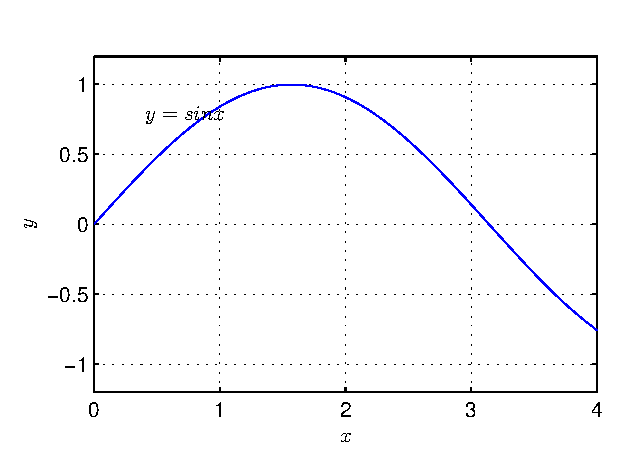
\includegraphics[scale=0.6]{./Pictures/matlabfigchg.eps}
\caption{matlab作图例}
\label{Figmatlab}
\end{figure}

图 \ref{Figmatlab} 中左图为matlab生成的eps图,右图为将左图中的s1,
纵横坐标名替换后的图片。可以把这一页放大几倍来看,图片依然非常清晰!
这就是矢量图的优势。
替换文字中如果有中文出现,因为dvips程序与cjk不兼容,
本论文模版的tex-dvi-pdf生成方式将不能用于含有dvips流程,使用dvips须使用cct方式,
具体请参考CTeX FAQ,有详细例子。

\subsection{子图的使用}
有些时候我们需要使用一级图放到一个大图中,这次版本也提供这种支持,具体实现代码如下:

{
\linespread{1}
\zihao{-5}\noindent
\begin{verbatim}
\begin{figure}[htb]
	\small
	%\centering
	\subfigure[子图1]{
		\begin{minipage}[b]{0.5\textwidth}
			\centering
			\label{fig:SubFigure1} %% label for second subfigure
			\includegraphics[scale=0.6]{./Pictures/matlabfig.eps}
		\end{minipage}}
		\subfigure[子图2]{
			\begin{minipage}[b]{0.5\textwidth}
				\centering
				\label{fig:SubFigure2} %% label for second subfigure
				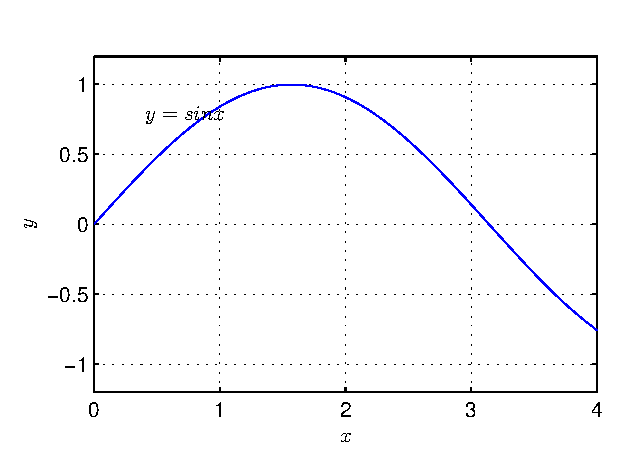
\includegraphics[scale=0.6]{./Pictures/matlabfigchg.eps}
			\end{minipage}}
			\caption{两个子图示例}
			\label{Fig:SubFigures}
		\end{figure}
\end{verbatim}
}
实现效果如图\ref{Fig:SubFigures}所示。

\begin{figure}[htb]
	\small
	%\centering
	\subfigure[子图1]{
		\begin{minipage}[b]{0.5\textwidth}
			\centering
			\label{fig:SubFigure1} %% label for second subfigure
			\includegraphics[scale=0.6]{./Pictures/matlabfig.eps}
		\end{minipage}}
	\subfigure[子图2]{
		\begin{minipage}[b]{0.5\textwidth}
			\centering
			\label{fig:SubFigure2} %% label for second subfigure
			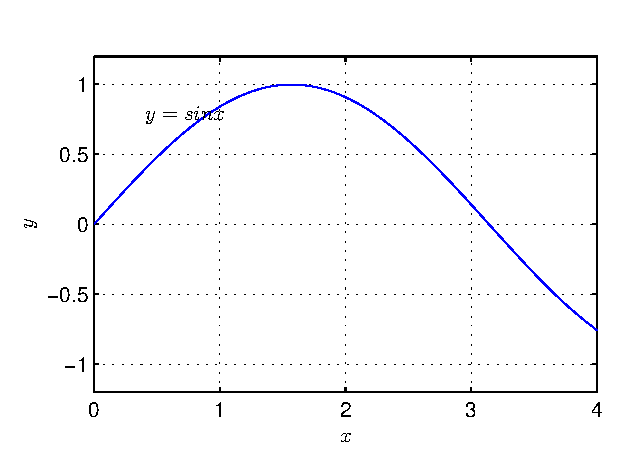
\includegraphics[scale=0.6]{./Pictures/matlabfigchg.eps}
		\end{minipage}}
		\caption{两个子图示例}
		\label{Fig:SubFigures}
\end{figure}

\section{插入表格}

\LaTeX 中建立表格比Word稍复杂一些,但表格的格式调整及效果比Word简单得多。

\subsection{普通表格的插入}

一个普通的插入表格代码如下所示,其生成的表格如表 \ref{Tabkeyword} 所示:

{
\linespread{1}
\zihao{-5}\noindent
\begin{verbatim}
{
\begin{table}[htb]
\zihao{5}
\caption{表格标题}
\label{Tabkeyword}
\centering
\begin{tabular}[t]{c|l|r|p{4cm}}
\hline
居中 & 靠左 & 靠右 & 靠左宽4cm\\
\hline
Center & Left & Right & Width=4cm\\
\hline
\end{tabular}
\end{table}
}
\end{verbatim}
}

\begin{table}[htb]
\zihao{5}
\caption{表格标题}
\label{Tabkeyword}
\centering
\begin{tabular}[t]{c|l|r|p{4cm}}
\hline
居中 & 靠左 & 靠右 & 靠左宽4cm\\
\hline
Center & Left & Right & Width=4cm\\
\hline
\end{tabular}
\end{table}

表格的使用一部分与图片相类似,比如开始的语句\verb+\begin{table}[htb]+,
以及结束的语句\verb+\end{table}+,与图片语句相比,除了把“figure”换成了
“table”,其它都相同。语句的含义也相同。

\verb+\zihao{5}+是把表格的字号改小一号,一般而言,表格字号应比正文字号小一号,
论文中的正文字号是小四号,那么表格中的字号就应该是五号字体。这个命令一定要写在
\verb+\begin{table}+ 的下方才能对该表格起作用。

\verb+\caption{表格标题}+是表格的标题,与图片标题格式相同,
会自动加到表格目录中去,如果表格标题太长,可以用
\verb+\caption[目录中的标题]{正文中的表格标题}+这种形式。

\verb+label{Tablekeyword}+与图片的标签相同,只要在正文中使用\\
\verb+\ref{Tablekeyword}+ 就可以在生成的文档中显示出表的编号,
同样,命令前后要各留一个空格,并且标签不能使用中文字符。

\verb+\centering+ 使整个表格居中放置。

\verb+\begin{tabular}[t]{c|l|r|p{4cm}}+是表格开始的标志,注意与
\verb+\begin+ \verb+{table}+区别开来,\verb+[t]+表示表格与其上方的正文行对齐方式是
行顶对齐,如果是\verb+[b]+则为行底对齐,这两种对齐方式可以在实际操作中试一下,
再做选择。\verb+{c|l|r|p{4cm}}+则代表这个表格各列的
对齐方式,c为居中,l为左对齐,r为右对齐,p\{4cm\}为该列宽度为4cm,并且左对齐。
中间接竖线“\verb+|+”则表示表格使用竖分隔线,如果没有这个竖线符号,对应位置就没有分隔线,
比如表 \ref{Tabkeyword} 就没有最左边和最右边的竖线。如果写为\verb+{|c|l|r|p{10cm}|}+,
就有最左边和最右边的竖线了。
如果不需要竖分隔线,则写为\verb+{clrp{10cm}}+
即可。要使用双竖线分隔线,就写为\verb+{c||c}+;还可以使用其它字条代替,
比如本模版的题名页中评阅人及答辩委员会信息就是利用的表格形式,它的分隔符是冒号“:”,
相应的命令就是\verb+{c@{:}c}+,即\verb+@{:}+。

\verb+\hline+就是画一条横线,如果没有写这一句命令,你会看到表格没有横分隔线。

表格内容是一行一行来填的,每一行结束使用断行符\verb+\\+,
同一行中不同列的元素用\&来分开。

\verb+\end{tabular}+表示表格结束。

\subsection{把表格换个样式}

上一小节介绍的方法生成的表格一般情况下可以用了,
但\LaTeX 的能力不止是做这样一个常规表格,
下面我们来利用booktabs-de\index{booktabs-de}扩展包来让表格看起来更professional一些。
这个扩展包的调用已经放在了本模版中了,使用本模版可以直接使用这种格式。
这个表格如表 \ref{Tab3Line} 所示。

{
\linespread{1}
\begin{table}[htb]
\zihao{5}
\caption{粗细线表格示例}
\label{Tab3Line}
\centering
\begin{tabular}[b]{cccc}
\toprule
长 & 宽 & 高 & 重量\\
(m) & (cm) & (mm) & (kg)\\
\toprule
1.234 & 5.676 & 332.876 & 3498.5\\
\midrule
548.4 & 23.43 & 34.98 & 923.8\\
\bottomrule
\end{tabular}
\end{table}
}

表 \ref{Tab3Line} 的实现代码如下所示:

{
\linespread{1}
\zihao{-5}\noindent
\begin{verbatim}
{
\linespread{1}
\begin{table}[htb]
\zihao{5}
\caption{粗细线表格示例}
\label{Tab3Line}
\centering
\begin{tabular}[b]{cccc}
\toprule
长 & 宽 & 高 & 重量\\
(m) & (cm) & (mm) & (kg)\\
\toprule
1.234 & 5.676 & 332.876 & 3498.5\\
\midrule
548.4 & 23.43 & 34.98 & 923.8\\
\bottomrule
\end{tabular}
\end{table}
}
\end{verbatim}
}

先解释一下这部分代码为什么会用一对大括号\{\}整个括起来。
如果要对文章中一部分内容的格式作调整,又不能影响到其它部分,
就使用一对大括号把要调整格式的部分括起来。
这里要调整的格式是行距。本论文的默认行距是1.5倍行距
\footnote{模版中的行距调整命令是$\backslash$linespread\{1.5\},
但并不是直接的1.5,这里有个换算,有兴趣的同学可以查看参考文献\cite{LaTeXshzh}},
在这里要把它调成单倍行距这个表格样式才比较美观,
因此就在最前使用\verb+\linespread{1}+命令把它的行距调整为单倍行距。
关于局部格式调整,在后面的《重点字符,醒目提醒》
一节中还将详细介绍,这里只对牵涉部分做简要说明。

这部分代码与普通表格代码的区别在于横线生成命令:\verb+\toprule+,\verb+\bottomrule+
都是比较粗的线条,\verb+\midrule+是比较细的线条。
此外,还有一个不完整线条命令,\verb+\cmidrule+,
该命令的使用类似下一小节要讲到的\verb+\cline+命令。

\subsection{有单元格合并的表格}

表格不可能总是一格归一格的。部分表格总是需要进行表格合并,
下面我就举一个表格合并的例子。\LaTeX 直接支持列合并,行合并则需要
扩展包multirow\index{multirow}的支持,本模版已经将该扩展包包含进去,可直接使用。
如表 \ref{TabComplex} 所示表格

\begin{table}[htp]
\zihao{5}
\caption{复杂表格示例}
\label{TabComplex}
\centering
\begin{tabular}[t]{|c|c|c|c|c|}
\hline
\multicolumn{2}{|c|}{我占了两列} & 第3列 & 第4列 & 第5列\\
\hline
\multirow{2}*{我占了两行} & 第二行第2列 & 第二行第3列 & \multicolumn{2}{|c|}{\multirow{2}*{我占了两行又两列}}\\
\cline{2-3}
& 第三行第2列 & 第三行第3列 & \multicolumn{2}{|c|}{} \\
\hline
\end{tabular}
\end{table}

表 \ref{TabComplex} 的实现代码如下:

{
\linespread{1}
\zihao{-5}\noindent
\begin{verbatim}
\begin{table}[htp]
\zihao{5}
\caption{复杂表格示例}
\label{TabComplex}
\centering
\begin{tabular}[t]{|c|c|c|c|c|}
\hline
\multicolumn{2}{|c|}{我占了两列} & 第3列 & 第4列 & 第5列\\
\hline
\multirow{2}*{我占了两行} & 第二行第2列 & 第二行第3列 & \multicolumn{2}{|c|}{\multirow{2}*{我占了两行又两列}}\\
\cline{2-3}
& 第三行第2列 & 第三行第3列 & \multicolumn{2}{|c|}{} \\
\hline
\end{tabular}
\end{table}
\end{verbatim}
}

\verb+\multicolumn{2}{|c|}{表格内容}+就是合并列的命令,参数2表示合并两列,
格式命令表示合并后的单元格居中对齐且两边有分隔竖线,注意在有分隔线时,分隔线符号
\verb+|+不要忘记。

\verb+\multirow{2}*{表格内容}+是合并行的命令,参数2表示合并两行,注意中间的*号。

注意同时合并行合并列时两个命令的嵌套方式,以及合并行情况下,除第一行外其它行的表示方式。
如合并两行两列时第二行的\verb+\multicolumn{2}{|c|}{}+。

\verb+\cline{2-3}+代表横线只划第二列与第三列,如果划2,3,5列,则写为\verb+\cline{2-3,5}+
\verb+\cmidrule+用法同\verb+\cline+。

\subsection{其它高级表格格式及扩展包简介}

如果需要实现表格左上角内有斜线的样式,
请使用slashbox\index{slashbox}扩展包并参考其自带帮助文档。

更复杂的表格,比如指定每一行的宽度,即可以借助盒子\cite{LaTeXshzh}来完成,
也可以借助扩展包array,tabularx等,具体实现代码此处不再详述,有兴趣的同学可参考文献
\cite{LaTeXshzh, Table:Lapo}以及扩展包内帮助文件。

\section{公式及其编号}

\LaTeX 出现之初的重要作用就是排版各种复杂的数学公式,关于数学公式的排版方法,
参考文献\cite{LaTeXshzh}中有一整章的内容来介绍各种公式的编辑。
我这里就偷个懒不写了,太长了,而且公式编辑我写不出我的特色来。

\LaTeX 的公式编辑效果远胜于Word中的公式编辑器,而且,使用LaTeX,
完全不用担心公式编辑器的版本问题,因为,这里公式就是用纯文本写的。
下面我举一个小小的公式例子来说明公式的编写及编号,如式 \ref{Equ:exm} 所示。

\begin{equation}
\label{Equ:exm}
c^2=a^2+b^2
\end{equation}

实现式 \ref{Equ:exm} 的代码如下所示:

{
\linespread{1}
\zihao{-5}\noindent
\begin{verbatim}
\begin{equation}
\label{Equ:exm}
c^2=a^2+b^2
\end{equation}
\end{verbatim}
}

\verb+\begin{equation}+与图片,表格很类似,开头都是一个环境开始命令,
只是这里的关键词是equation\index{equation}。

\verb+label{Equ:exm}+是给公式一个编号,以便在文中引用。该公式编号由\LaTeX 负责,
一般不需人工干预。

\verb+\ref{Equ:exm}+就是文中引用公式的命令。

\section{索引}

索引比较简单,只要在你想放索引的位置放上命令\\
\verb+\index{索引名}+,\\
然后文后面的索引列表中就出现“索引名”这个条目,并且有它的页码,
索引支持中文,英文字符。
如果文中有多处同名索引,这个表中都会把它们按字母表顺序列出来。
很方便的,你想在哪里插入索引就在哪里插入索引,完全不必考虑索引列表的事。

\section{参考文献}

前面介绍参考文献时就提到,只要准备好自己的参考文献数据库,
在引用参考文献时只需要利用\verb+\cite{tag}+就能把相应的参考文献引上。
这里的tag就是在参考文献数据库中各参考文献定义的标签,不能含有中文字符。
多个文献,则中间用英文逗号分开如\verb+\cite{tag1,tag2}+。
不需要考虑引用顺序,\LaTeX 会替你打理好一切。

如果想用形如“文献[1]提出XXX”的格式,则使用如下代码。

{\noindent\zihao{-5}\verb+文献[\citenum{tag}]提出+}

该模版已经把各类参考文献的列出格式按毕业论文要求调整好,不需要再修改。

如果你想了解更多参考文献格式调整的信息,请参考扩展包natbib\index{natbib},custom-bib\index{custom-bib}
自带的帮助文档。本次修订版新增的第5章也专门会对参考文献的格式校调问题进行大篇幅介绍。

\section{脚注}

有些时候需要使用脚注,\LaTeX 的脚注功能也是很方便的,
只要在你想要放一个脚注的地方用命令\verb+\footnote{脚注内容}+即可,
脚注内容长度不限,脚注编号\LaTeX 会替你操心。
你要做的,只是写好这个脚注的内容。

对于表格加脚注,就像表 \ref{ChapsecList} 显示效果那产,则稍显麻烦一点,需要把表格放进一个minipage里去。
关键代码如下:

{
\linespread{1}
\zihao{-5}\noindent
\begin{verbatim}
\begin{table}
……
\centering
\begin{minipage}[c]{10cm}
\centering
\begin{tabular}
……
\end{tabular}
\end{minipage}
……
\end{table}
\end{verbatim}
}

\verb+\begin{minipage}[c]{10cm}+表示创建一个内部居中对齐的,
宽度为10cm的小页面,这个宽度要根据其内部表格宽度来确定,
这样出来的脚注才美观。

\section{重点字符,醒目标示}

有的时候需要对某些内容做一个醒目标示,比如改变字体啦,字体加粗啦。
这个时候首先要把需要改变格式的部分用一对大括号
\footnote{要使用英文字符的大括号\{\}}括起来。
然后在头上写上字体字号之类的命令。就像这样

我这一段话里有{\bfseries 加粗},
{\kaishu\bfseries 有楷体并加粗},有{\heiti 黑体},还有{\zihao{3}三号字}字体。

这一句话的实现代码如下:

{
\linespread{1}
\zihao{-5}\noindent
\verb+我这一段话里有{\bfseries 加粗},{\kaishu\bfseries 有楷体并加粗},有{\heiti 黑体},还有{\zihao{3}三号字}字体。+
}

在\LaTeX 中可以用的字体有{\songti 宋体}\verb+\songti+,{\fangsong 仿宋}\verb+\fangsong+,
{\kaishu 楷体}\verb+\kaishu+,{\heiti 黑体}\verb+\heiti+,
{\youyuan 幼圆}\verb+\youyuan+,{\lishu 隶书}\verb+\lishu+六种。字号命令是\verb+\zihao{1}+字号从
1,-1,2,-2,一直到8号字,前面带负号表示小号字,比如-4就是小四号字体。
7,8两个字号没有小号字对应。

关于加粗字体命令\verb+\bfseries+,对英文字符只要使用\verb+\bf+即可,
中文字符应使用\verb+\bfseries+。

关于字体效果的设置,更多内容参见CTeX自带的帮助文档ctex.pdf。

如果想使用更多的字体,比如微软雅黑,请自行网络搜索方法,自己生成字体文件并关联上即可。
CTeX提供的六种字体,一般情况下已经足够使用。






\ZJUbackmatter
%%%%%%%%%%%%%%%%%%%%%%%%%%%%%%
%% 参考文献
%%%%%%%%%%%%%%%%%%%%%%%%%%%%%%
\ZJUthesisbib{thesisbib}

%%%%%%%%%%%%%%%%%%%%%%%%%%%%%%
%% 附录
%%%%%%%%%%%%%%%%%%%%%%%%%%%%%%
% \appendix
% \chapter{附录A}

这是附录A的内容。

\chapter{附录B}

这是附录B的内容。



%%%%%%%%%%%%%%%%%%%%%%%%%%%%%%
%% 索引
%%%%%%%%%%%%%%%%%%%%%%%%%%%%%%
% \ZJUindex

%%%%%%%%%%%%%%%%%%%%%%%%%%%%%%
%% 发表论文目录
%%%%%%%%%%%%%%%%%%%%%%%%%%%%%%
\begin{publications}
\begin{enumerate}
\item{第一篇}
\item{第二篇}
\end{enumerate}
\end{publications}


\end{document}
